\documentclass{sigplanconf}
\usepackage{version}
\usepackage{graphicx}
\usepackage{amsmath}
\usepackage{mathptmx}
\usepackage{style/code}
\usepackage{style/utils}


% -----------------------------------------------------------------------------
\begin{document}
\title	{Work Efficient Higher-Order Vectorisation}

\authorinfo{
  \shortstack{%
    Ben Lippmeier$^\dagger$            \and
    Manuel M. T. Chakravarty$^\dagger$ \and 
    Gabriele Keller$^\dagger$           \and 
    Roman Leshchinskiy$^\dagger$       \and
    \\[4pt]
    Simon Peyton Jones$^\ddagger$
  }
}{
  \vspace{5pt}
  \shortstack{
    $^\dagger$Computer Science and Engineering \\
    University of New South Wales, Australia \\[2pt]
    \textsf{\{benl,chak,keller,rl\}@cse.unsw.edu.au}
  }
  \and
  \shortstack{
    $^\ddagger$Microsoft Research Ltd \\
    Cambridge, England \\[2pt]
    \textsf{\{simonpj\}@microsoft.com}
  }
}

\conferenceinfo{ICFP'12,} {September 9--15, 2012, Copenhagen, Denmark.}
\CopyrightYear{2012}
\copyrightdata{978-1-4503-1054-3/12/09}

\maketitle
\makeatactive

% -----------------------------------------------------------------------------
\begin{abstract}
Existing approaches to \emph{higher-order vectorisation}, also known as \emph{flattening nested data parallelism,} do not preserve the asymptotic work complexity of the source program. Straightforward examples, such as sparse matrix-vector multiplication, can suffer a severe blow-up in both time and space, which limits the practicality of this method. We discuss why this problem arises, identify the mis-handling of index space transforms as the root cause, and present a solution using a refined representation of nested arrays. We have implemented this solution in Data Parallel Haskell (DPH) and present benchmarks showing that realistic programs, which used to suffer the blow-up, now have the correct asymptotic work complexity. In some cases, the asymptotic complexity of the vectorised program is even better than the original.
\end{abstract}

\category
	{D.3.3}
	{Programming Languages}
	{Language Constructs and Features---Concurrent programming structures; Polymorphism; Abstract data types}

\terms
	Languages, Performance

\keywords
	Arrays, Data parallelism, Haskell


% -----------------------------------------------------------------------------
%!TEX root = ../Main.tex
\section{Introdution}

The Haskell library ecosystem is blessed with a multitude of libraries for writing streaming data flow programs. Stand out examples include iteratee CITE, enumerator CITE, conduit CITE and pipes CITE. These libraries are based around ... and more recent examples such as pipes provide a useful set of algebraic equivalences that give a clean mathematical structure to the provided mathemetical structure.

Libraries such as iteratee and enumerator are typically used to deal with data sets that do not fit in main memory, as the constant space guarantee ensures that the program will run to completion without suffering an out-of-memory error. However, current computing platforms use multi-core processors, the programming models provided by such streaming libraries do not also provide a notion of \emph{parallelism} to help deal with the implied amount of data. They also lack support for branching data flows where produced streams can be consumed by several consumers without the programmer needing to had fuse them.

We provide several techniques that increase the scope of programs that can be written in such libraries. Our target applications concern \emph{medium data}, meaning data that is large enough that it does not fit in the main memory of a normal desktop machine, but not so large that we require a cluster of multiple physical machines. For a lesser amount of data one could simply load the data into main memory and use an in-memory array library such as CITE or CITE. For greater data one needs to turn to a distributed system such as Hadoop or Spark and deal with the unreliable network and lack of shared memory. Repa Flow targets the sweet middle ground.

We make the following contributions:

\begin{itemize}
\item Our parallel data flows consist of a bundle of streams, where each stream can process a separate partition of a data set on a separate processor core.

\item Our API uses polarised flow endpoints (@Sources@ and @Sinks@) to ensure that programs run in constant space. We demonstrate how this standard technique can be extended to branching data flows, where produced flows are consumed by multiple consumers.

\item The data processed by our streams is chunked so that each operation processes several elements at a time. We show how to design the core API in a generic fashion so that chunk-at-a-time operators can interoperate smoothly with element-at-a-time operators.
\TODO{We don't support leftovers}

\item We show how to use Continuation Passing Style to provoke the Glasgow Haskell Compiler into applying stream fusion across chunks processed by independent flow operators. For example, the map-map fusion on flows arises naturally from map-map fusion rule on chunks (arrays) of elements.
\end{itemize}

Our work is embodied in Repa Flow, which is available on Hackage. \TODO{Specify the relationship to previous work on Repa}. This is a new layer on the original delayed arrays of our original Repa library.



\section{Representation, Fusion, and Code Explosion}
\label{section:problem}

\begin{figure}
\begin{small}
\begin{code}
data Array sh e = Manifest sh (Vector e)
                | Delayed  sh (sh -> e)

class Shape sh where
   toIndex      :: sh -> sh -> Int
   fromIndex    :: sh -> Int -> sh
   size         :: sh -> Int
   ...more operations...
data DIM1 = DIM1 !Int
data DIM2 = DIM2 !Int !Int
...more dimensions...

index :: Shape sh => Array sh e -> sh -> e
index (Delayed sh f)    ix = f ix
index (Manifest sh vec) ix = indexV vec (toIndex sh ix)

delay :: Shape sh => Array sh e -> (sh, sh -> e)
delay (Delayed  sh f)   = (sh, f)
delay (Manifest sh vec) 
 = (sh, \ix -> indexV vec (toIndex sh ix))

map :: Shape sh => (a -> b) -> Array sh a -> Array sh b
map f arr = let (sh, g) = delay arr 
            in  Delayed sh (f . g)

zipWith :: Shape sh => (a -> b -> c) 
        -> Array sh a -> Array sh b -> Array sh c
zipWith f arr1 arr2
 = let  (sh1,  f1)       = delay arr1
        (_sh2, f2)       = delay arr2
        get ix          = f (f1 ix) (f2 ix)
   in   Delayed sh1 get

force :: Shape sh => Array sh e -> Array sh e
force arr 
 = unsafePerformIO
 $ case arr of
    Manifest sh vec    
     ->     return  $ Manifest sh vec
    Delayed sh f    
     -> do  mvec    <- unsafeNew (size sh)
            fill (size sh) mvec (f . fromIndex sh)
            vec     <- unsafeFreeze mvec
            return  $ Manifest sh vec
\end{code}
\caption{Essential Repa Version 1 Definitions}
\label{figure:Repa1}
\end{small}
\end{figure}

We start by reviewing the design problems of original Repa library. A simplified version of the core definitions of Repa~1~\cite{Keller:Repa} is in Figure~\ref{figure:Repa1}. Repa~2 extends the @Array@ type to support more efficient convolutions~\cite{Lippmeier:Stencil}, which we discuss in \S\ref{section:Explosion}.

Repa~1 introduced \emph{delayed arrays} to fuse multiple array operations, and minimise the overhead of \emph{index-space transforms}. Delayed arrays are represented by a function from indices to array elements, as we see in the definition of @Array@ Figure~\ref{figure:Repa1}. Delayed arrays contrast with \emph{manifest} arrays, which are represented as contiguous blocks of unboxed values. Fusion of operations on delayed arrays amounts to function composition, as we see in the definition of @map@. This gives us the map/map fusion rule, @map f . map g = map (f . g)@, for free and works similarly for many other operations, including index space transforms such as permutation, replication, slicing, and so on.

The elements of a multi-dimensional @Manifest@ array are stored in row-major order in a flat, one-dimensional @Vector@. The @Shape@ class holds operations to convert between higher-dimensional index types, such as @DIM2@, and the flat representation. In particular, the @toIndex@ and @fromIndex@ functions convert between higher-dimensional and linear indices, and @size@ yields the total number of elements in an array of the given shape. Based on the methods of the @Shape@ class, the function @index@ retrieves a single element from an array, and @delay@ produces an array's shape together with an indexing function to move to the delayed representation. (The function @indexV@ indexes into the flat @Vector@.)

As stated in the introduction, although Repa 1 \& 2 can produce efficient code on both sequential and parallel machines~\cite{Keller:Repa,Lippmeier:Stencil}, they have some significant shortcomings, which we review next.


% -----------------------------------------------------------------------------
\subsection{Problem 1: Not Applying {\texttt force}}
\label{section:force}

To illustrate the problems with Repa 1, we will reuse the example from the introduction:
%
\begin{small}
\begin{code}
    doubleZip :: Array DIM2 Int -> Array DIM2 Int 
              -> Array DIM2 Int
    doubleZip arr1 arr2
     = map (* 2) $ zipWith (+) arr1 arr2
\end{code}
\end{small}

\eject
By inlining the definitions from Figure~\ref{figure:Repa1} and simplifying, we see that the composition of @map@ and @zipWith@ fuses to produce the following:
%
\begin{small}
\begin{code}
    let (sh1,  f1) = delay arr1
        (_sh2, f2) = delay arr2
        get ix     = (f1 ix + f2 ix) * 2
    in Delayed sh1 get
\end{code}
\end{small}
%
The problem is that the array returned by @map@ is not a \emph{manifest} array, so is not represented as real unboxed data in a contiguous block of memory. Instead, it is a \emph{delayed} array, represented by a function that takes an array index and computes each element on the fly. The fused code immediately builds a new @Delayed@ array without doing any actual work. This is problematic if the consumer of a delayed array uses elements multiple times. The elements will be recomputed each time, so sharing of results is lost along with runtime performance.

If we desire an array represented by real data, then we should use Repa's @force@ function, which turns a delayed array into a manifest array by executing loop-based parallel array filling code. We would use it in @doubleZip@ as follows:
%
\begin{small}
\begin{code}
    doubleZip arr1 arr2
     = force $ map (* 2) $ zipWith (+) arr1 arr2
\end{code}
\end{small}
%
The code here fuses @map@ and @zipWith@ by building a new Delayed array as before. It then fills a freshly-allocated @Manifest@ array, \emph{in parallel}, using the element-generating function stored in the new @Delayed@ array. In other words, the compiled code will contain an unfolding of the imperative loop provided by @force@, where the body performs the per-element function, here @(f1 ix + f2 ix) * 2@, where @f1@ and @f2@ retrieve elements from the two input arrays. 

Although our entire approach to parallel array programming hinges on the correct use of @force@, the type presented in the Repa~1 API documentation was rather uninformative:

\begin{small}
\begin{code}
  force :: Shape sh => Array sh a -> Array sh a
  -- Force an array, so that it becomes Manifest.
\end{code}
\end{small}
%
From its type alone, @force@ looks like an instance of the identity function. This coupled with the rather cryptic comment, led many users to overlook @force@ entirely. Poor documentation aside, our foundational view that ``a type is a name for a set of values'' was of no help in expressing the fact that ``if you don't use this function your program will be really slow''. 


% -----------------------------------------------------------------------------
\subsection{Problem 2: Runtime Representation Tests}
\label{section:rep-tests}

The version of @doubleZip@ using @force@ produces fused, loop-based code, but is still slower than a straightforward imperative version. This is because the @Array@ type has two data constructors, @Delayed@ and @Manifest@, so indexing functions must perform a run-time test to distinguish between them. This is a catastrophe if the test is in an inner loop, which is the native environment for indexing functions. In some cases GHC can lift such tests out of loops, but in general such transformations are unsound, because they can change strictness properties if the loop can perform no iterations.

Tantalisingly, the representation of an array at a particular program point does not change from run to run. The programmer always knows which representation is expected --- but, in Repa 1 \& 2 they lack a convenient way to express that knowledge. For example, if we know that only manifest arrays will be passed to @doubleZip@, then we should reify this fact by using explicit pattern matching:
\par
\begin{small}
\begin{code}
  doubleZip arr1@Manifest{} arr2@Manifest{}
   = force $ map (* 2) $ zipWith (+) arr1 arr2
\end{code}
\end{small}
%
While this version runs fast, it is awkward due to the implicit precondition: we need to ensure that all callers of @doubleZip@ force the arguments to ensure that they are manifest. 

The test for array representation is not the only run-time test that tends to be needlessly performed in an inner loop. An array also contains size information such as its width and height, which is often used in each iteration. As these are boxed @Int@ values, a loop might repeatedly unbox them, wasting cycles. To ensure the values are unboxed only once, in the preamble of the loop, we need to place a demand on them at the function entry point. We typically do this using bang patterns in the pattern that matches @Manifest@, and it turns out we also want to demand the flat vector to ensure its components are unboxed as well:
%
\begin{small}
\begin{code}
  doubleZip arr1@(Manifest !_ !_) arr2@(Manifest !_ !_)
  = force $ map (* 2) $ zipWith (+) arr1 arr2
\end{code}
\end{small}
%
Finally, @doubleZip@ runs as fast as a hand-written imperative loop. Unfortunately, the optimisations require reasoning that is not obvious from the source program, demand a deeper understanding of the compilation method than most users will have, and add a precondition that is not captured in the function signature.


% -----------------------------------------------------------------------------
\subsection{Problem 3: Inlining and Code Explosion}
\label{section:Explosion}

In a FORTRAN or C program, the programmer writes explicit loops. In Repa, the programmer never writes loops; the loops are in library functions. With respect to Figure~\ref{figure:Repa1}, the key loop is in the definition of @fill@, which is called by @force@. The loop code itself is too big to include here, but see \cite{Lippmeier:Stencil} for a full definition. The array operations such as @map@, @zipWith@ and so on, build @Delayed@ arrays by composing functions, but do not contain loops.

How does this turn into efficient code? Consider the last, most efficient version of @doubleZip@. Inlining @zipWith@, @map@, @delay@, and @force@, then simplifying yields:
\par
\begin{small}
\begin{code}
  doubleZip (Manifest !sh1 !vec1) (Manifest !_sh2 !vec2) 
   = unsafePerformIO 
   $ do mvec <- unsafeNew (size sh1) 
        fill (size sh1) mvec
          (\ix -> (indexV vec1 ix + indexV vec2 ix) * 2)
        vec <- unsafeFreeze mvec
        return $ Manifest sh1 vec
\end{code}
\end{small}
%
The pattern matching in @zipWith@'s calls to @delay@ are cancelled by the explicitly @Manifest@ arrays; the @Delayed@ array produced by @zipWith@ is canceled by the pattern match in @map@'s use of @delay@; and so on. When the definition of @fill@ is inlined, we get a tight loop, in which the output is built directly from the input vectors (@vec1@, @vec2@) without any intermediates.

Clearly, this fusion depends critically on (a) aggressive inlining and (b) cancellation of statically-visible array construction and pattern matching.  However, for efficient stencil convolution, we developed a more complex array representation~\cite{Lippmeier:Stencil}, similar to this:
\par
\begin{small}
\begin{code}
  data Array sh a 
    = Array { arrayExtent  :: sh
            , arrayRegions :: [Region sh a] }
\end{code}
\end{small}
%
Rather than just being @Manifest@ or @Delayed@, these arrays consist of a list of rectangular \emph{regions}. Each region has its own element-generating function, which is used to speed up the handling of boundary conditions.

Alas, this representation is fatal for the inline-and-cancel story outlined above. This is because the list @arrayRegions@ must be processed by a \emph{recursive} function, and compilers (including GHC) are rightly cautious about unrolling recursive functions. In a typical application the programmer knows the exact number of regions at any program point, say four boundaries and a central region. Unrolling five times here would be perfect, but the compiler does not know this.

\eject
To make this work, we ended up manually unrolling code in the library functions, by pattern matching on the region list. Here is a typical chunk of Repa 2 library code:
\par
\begin{small}
\begin{code}
  forceWith2 :: (Int -> a -> IO ())
             -> Array DIM2 a -> IO ()
  forceWith2 write arr
   = case arr of
      Array sh [r1]
       -> do fillRegion2P write sh r1
      Array sh [r1, r2]
       -> do fillRegion2P write sh r1
             fillRegion2P write sh r2
      Array sh [r1, r2, r3]
       -> do fillRegion2P write sh r1
             fillRegion2P write sh r2
             fillRegion2P write sh r3
      ...
      Array sh regions
       ->    mapM_ (fillRegion2P write sh) regions
\end{code}
\end{small}       
%
The details are not important, but it should be clear from the form how gruesome this is:
\begin{itemize}
\item The library only efficiently accommodates a maximum number of regions. If we use the final alternative of @forceWith2@ above, then the code will not fuse.
\item There is much repetition in the library code.
\item The library functions become very large because of the duplication, but they must still be inlined!
\end{itemize}
%
Aggressive use of @INLINE@ pragmas produces enormous intermediate programs, which we hope will then shrink radically through construction/pattern-matching cancellation. Sadly, this cancellation does not always happen; imagine that the @arr@ argument of @forceWith2@ above turned out to be lambda-bound, so that the @case@ remained in the residual program.


% -----------------------------------------------------------------------------
\subsection{Summary}

The fundamental problem with Repa 1 \& 2 is the following: at a particular point in the code, the programmer typically has a clear idea of the array representation they desire. For example, it may consist of three regions, left edge, middle, right edge, each of which is a delayed array. Although this representation is statically known to the programmer, it is invisible in the types and only exposed to the compiler if very aggressive value inlining is used. Moreover, the programmer's typeless reasoning can easily fail, leading to massive performance degradation.

The solution is to expose static information about array representation to Haskell's main static reasoning system; its type system.


\clearpage{}
% -----------------------------------------------------------------------------
\section{Baseline Representation of Nested Arrays} 
\label{section:naive-flat}
A key idea of Blelloch's vectorisation transformation is to flatten the representation of nested arrays, as well as the parallelism itself. More precisely: an array $A$ of sub-arrays $A_0, A_1, ..., A_{n-1}$ (each with its own length) is represented by (a) a single long array of data, $D = [A_0, A_1, ..., A_{n-1}]$ all laid out in one contiguous block, and (b) a \emph{segment descriptor} that gives the length of each $A_i$ in the data block $D$.  We call $A_i$ the \emph{segments} of $A$.  The idea is to divide the data block $D$ evenly over the processors, and process each chunk independently in parallel. This provides both excellent granularity and excellent data locality, which is intended to satisfy the second part of our Complexity Goal. There is some book-keeping to do on the segment descriptor; generating that book-keeping code is the job of the vectorisation transformation.

Figure~\ref{figure:OldArrayRepresentation} gives the representation of nested arrays in Haskell, using GHC's \emph{data families}~\cite{chak-etal:ATs}.  An array of type @(PA e)@ is represented by a pair @PA n d@, where @n@ is the length of the array, and @d :: PData e@ contains its data.  The representation of @PData@ is type-dependent --- hence, its declaration as a @data family@.  When the argument type is a scalar, matters are simple: @PData Int@ is represented merely by a @Vector Int@, which we take as primitive here\footnote{It is provided by the @vector@ library.}. Arrays of @Char@ are represented similarly. On the other hand, the data component of a \emph{nested array}, with type @PData (PA e)@ is represented by a pair of a segment descriptor of type @Segd@, and the \emph{data block} of type @PData e@.  
The segment descriptor @Segd@ has two fields, @lengths@ and @indices@.  The latter is just the scan (running sum) of the former, but we maintain both in the implementation to avoid recomputing @indices@ from @lengths@ repeatedly.  Each is a flat @Vector@ of @Int@ values.

Using the example from the previous section, the array @xss1@ has type @(PA (PA Char))@ and is represented like this:
%
\begin{small}
\begin{code}
   replicates [3 1 2 1] [[A B] [C D E] [F G] [H]]
   = [[A B] [A B] [A B] [C D E] [F G] [F G] [H]] 
 ----------------------------------------------- (ARR0)
  PA 7 (PNested
   (Segd lengths: [2 2 2 3 2 2  1] 
         indices: [0 2 4 6 9 11 13])
   (PChar [A B A B A B C D E F G F G H]))
\end{code}
\end{small}
%
We show the \emph{logical value} of the array above the line, and its \emph{physical representation} below. The representation is determined by the data type declarations in Figure~\ref{figure:OldArrayRepresentation}.  The result array is built with an outer @PA@ constructor, pairing its length, @7@, with the payload of type @PData (PA Char)@.  From the @data instance@ for @PData (PA e)@, again in Figure~\ref{figure:OldArrayRepresentation}, we see that the data field consists of a @PNested@ constructor pairing a segment descriptor with a value of type @PData Char@.  Finally, the latter consists of a @PChar@ constructor wrapping a flat @Vector@ of @Char@ values.

The process continues recursively in the case of deeper nesting: the reader may care to write down the representation of a value of type @PA (PA (PA Int))@. We will see an example in \S\ref{section:PlainReplicate}.

Now the problem with @replicates@ becomes glaringly obvious. The baseline representation of arrays, which was carefully chosen to give good locality and granularity, is \emph{physically incapable of representing the sharing between subarrays in the result} --- and losing that sharing leads directly to worsening the asymptotic complexity. It is not possible to simply eliminate the call to @replicates@ itself, because this function plays a critical role in vectorisation. In the example from \S\ref{section:problem}, @replicates@ distributes shared values from the context of the outer computation (@zipWithP mapP@) into the inner computation (@mapP indexP@). Since we cannot eliminate @replicates@, the only way forward is to change the representation of nested arrays.





\begin{figure}
\begin{center}
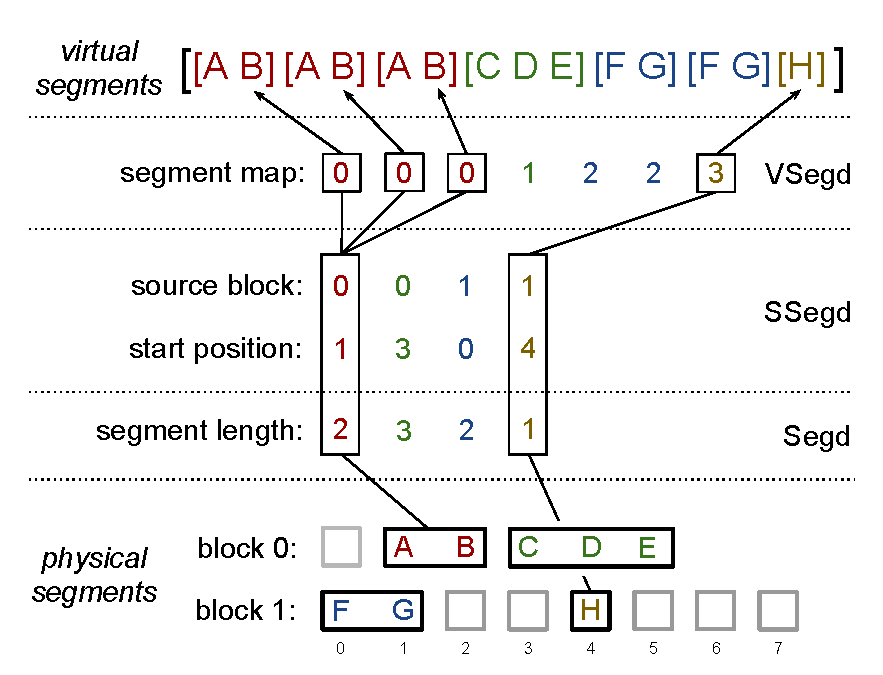
\includegraphics[scale=0.6]{figures/NewArrayRep}
\caption{New Array Representation}
\end{center}
\label{figure:NewArrayPicture}
\end{figure}

\eject{}

% -----------------------------------------------------------------------------
\section{New Representation of Nested Arrays}
\label{section:Segds}

The new array representation must support all index space transforms that vectorisation introduces, in a way that allows the vectorised program to have the same asymptotic complexity as the original unvectorised program. This is up to \emph{containment} which is discussed in \S\ref{section:PackCombine}. In most cases this comes down to having the same complexity as the direct representation, where nested arrays are stored as flat arrays of pointers to more arrays. However, we cannot use this representation as described, because it would lose the granularity and data locality benefits of the baseline segmented representation. We need the best of both worlds.


% -----------------------------------------------------------------------------
\subsection{Physical, Virtual and Scattered Segments}
An example array with the same value as @ARR0@ is shown in Figure~\ref{figure:NewArrayPicture}. Our new representation has the following key features:
\begin{enumerate}
\item   We distinguish between \emph{physical} and \emph{virtual} segments. Physical segments consist of real element data in memory, while virtual segments are defined by mapping onto physical segments. This distinction enables us to define nested arrays with repeated segments without copying element data.

\item   The physical segments of a nested array may now be scattered through several data blocks, instead of being contiguous. Although we prefer segments to be contiguous for locality reasons, we must also allow them to be scattered, so that we can filter a nested array without copying element data.
\end{enumerate}
In the example, there are seven virtual segments defined from four physical segments. The physical segments lie scattered in two data blocks. We will see why we need to allow physical segments to lie in separate data blocks in \S\ref{section:Append}. The overall segment descriptor is now stratified into three layers: @VSegd@ (virtual segments); @SSegd@ (scattered segments) and plain @Segd@ (contiguous segments). In our terminology, we refer to all of @VSegd@, @SSegd@ and @Segd@ as ``segment descriptors'', individually or grouped together. At the bottom layer, @Segd@ gives the length of each segment, and would be sufficient to describe the array if all segments were contiguous in a single block. The @SSegd@ gives the index of the source data block, and starting position for each physical segment in its block. The @VSegd@ provides the mapping between virtual and physical segments. We have elided the @indices@ field from the diagram for clarity, but also include this in our new array representation as part of the @Segd@.


\clearpage{}
% -----------------------------------------------------------------------------
\subsection{The Concrete Definition}
\label{section:Representation}

\begin{figure}
\begin{small}
\begin{code}
data PA e = PA { length :: Int, pdata :: PData e }
data family   PData  e
data family   PDatas e
data instance PData  Int  = PInt   (Vector Int)
data instance PDatas Int  = PInts  (Vector (Vector Int))
data instance PData  Char = PChar  (Vector Char)
data instance PDatas Char = PChars (Vector (Vector Char))

data instance PData (PA e)
 = PNested { vsegd :: VSegd, pdatas :: PDatas e }

data instance PDatas (PA e)
 = PNesteds (Vector (PData (PA e)))

data VSegd  -- Virtual-segment descriptor.
 = VSegd { segmap  :: Vector PsId, ssegd :: SSegd }

data SSegd  -- Scattered-segment descriptor.
 = SSegd { sources :: Vector DbId, starts :: Vector Int }
         , segd    :: Segd }

data Segd   -- Contiguous-segment descriptor.
 = Segd  { lengths :: Vector Int, indices :: Vector Int }

type PsId = Int  -- Physical segment Id, indexes 'sources'
type DbId = Int  -- Data block Id, indexes 'pdatas'
\end{code}
\end{small}
\caption{Definition of the New Array Representation}
\label{figure:NewArrayRepresentation}
\end{figure}

The concrete definition of our new array type is given in Figure~\ref{figure:NewArrayRepresentation}. The data type @PA@ is unchanged from Figure~\ref{figure:OldArrayRepresentation}: a pair of a length and payload. The instances for @PData Int@ and @PData Char@ are also unchanged. The difference is in the representation of nested arrays:
\begin{small}
\begin{code}
  data instance PData (PA a)
   = PNested { vsegd  :: VSegd, pdatas :: PDatas a }
\end{code}
\end{small}
The payload is now a @PDatas@ (plural) rather than @PData@. Where @PData@ represents a single data block, @PDatas@ represents a vector of data blocks. We use the type @DbId@ (short for data-block identifier) to index this vector of @PData@ values. 

The @vsegd@ field holds the \emph{virtual segment descriptor}.  It consists of a vector of physical segment identifiers (@segmap@), and a scattered segment descriptor (@ssegd@). The @segmap@ maps virtual segments onto physical segments and corresponds 1-1 with the outer level of the array being represented. In Figure~\ref{figure:NewArrayPicture}, we have seven entries in this map and seven subarrays in the overall nested array.

Each entry in the @segmap@ is a \emph{physical segment identifier}, of type @PsId@. A @PsId@ is the index of one of
the physical segments described by the @SSegd@ and @Segd@ types. Crucially, the @segmap@ can contain repeated use of the same physical segment. In Figure~\ref{figure:NewArrayPicture} we have used @[0 0 0 1 2 2 3]@ to indicate three copies of the first physical segment, one copy of the second, and so on. This is how we represent the sharing defined by @replicates@. Note that we can not just store the replication counts @[3 1 2 1]@ directly because we must be able to map virtual segments to physical segments in constant time.

The @SSegd@ and @Segd@ together describe the physical segments. Together they contain four vectors, \emph{all of the same length}, two of them nested inside the @segd@ field. The @sources@ vector gives the data block identifier, @DbId@, which is the index of one of the data blocks in the @pdatas@ field. The next two, @starts@ and @lengths@, give the starting position and length of the physical segment in that data block. Finally @indices@ is, as before, a cached copy of the scan (accumuated sum) of @lengths@. Keeping @SSegd@ and @Segd@ separate is helpful when optimising vectorised code for absolute performance, which we discuss in \S\ref{section:Pragmatics}. 

Finally, the array representation must obey the following invariants:

\begin{enumerate}
\item	The lengths of the @sources@, @starts@, @lengths@, and @indices@ fields must all be the same.

\item	Every @PsId@ in the @segmap@ must be less than the length of the @sources@ field. 

\item	Each @DbId@ in @sources@ must be less than the length of the @pdatas@ vector.

\item	Each element of @starts[i]@ must be less than the length of @pdatas[sources[i]]@.

\item	The @indices@ field is equal to @init (scan (+) 0 lengths)@.

\item	All physical segments defined by the @SSegd@ and @Segd@ types must be reachable from the @segmap@. More precisely, the set of physical segment identifiers in the @segmap@ must cover @[0..np-1]@, where @np@ is the length of the @starts@, @sources@, @lengths@, and @indices@ fields.

\item	All @pdata@ blocks must be reachable from the @sources@ field.  More precisely, the set of @sources@ must cover @[0..nb-1]@, where @nb@ is the length of the @pdatas@ vector.
\end{enumerate}

Invariants 1 to 4 are standard well-formedness conditions. Invariant 2 ensures that each physical segment identifier points to a real physical segment. Invariant 3 ensures that each data block identifier points to a real data block. Invariant 5 says that @indices@ is precomputed from @lengths@. The reason for this is discussed in \S\ref{section:Pragmatics}. Invariants 6 and 7 ensure that the size of the internal structure of the array is bounded by the number of virtual segments, which is necessary for the complexity bound on @append@ (\S\ref{section:Append}). Invariant 7 is also needed to ensure that the parallel implementation of reductions such as @sum@ do not duplicate work (\S\ref{section:Reduction}). However, an implementation may be able to relax these last two invariants in certain cases (\S\ref{section:Pragmatics}).


% -----------------------------------------------------------------------------
\subsection{Replicates again}
\label{section:Replicates}
Now let us implement @replicates@ using our new array representation. The start is easy, because the result @PA@ array must be built with a @PA@ constructor:
\par
\begin{small}
\begin{code}
 replicates :: Vector Int -> PA e -> PA e
 replicates ns arr = PA (sum ns) (replicatesPR ns arr)
\end{code}
\end{small}
\par
\noindent
The real work is in @replicatesPR@.  But now we encounter a slight problem: since the representation of @PData@ is indexed by the element type @e@, we require a type-indexed function to operate over @PData@ values.  That is, we need a type class, with an instance for @Int@ and an instance for @(PA e)@:
\begin{small}
\begin{code}
 class PR e where
   replicatesPR :: Vector Int -> PData e -> PData e
   ...more methods...

 instance PR Int where
   replicatesPR = replicatesI
   ...
 instance PR e => PR (PA e) where
   replicatesPR = replicatesPA
   ...
\end{code}
\end{small}
The @PR@ (Parallel Representation) class is given in Figure \ref{figure:NewArrayOperators}, and conveniently collects all the necessary primitive operations over arrays.  We will see more of them in this section, but @replicatesPR@ is one. So, in fact, we lied: the types of @replicates@ and @replicatesPR@ are overloaded thus:
\par
%
\begin{small}
\begin{code}
 replicates   :: PR e => Vector Int -> PA e    -> PA e
 replicatesPR :: PR e => Vector Int -> PData e -> PData e
\end{code}
\end{small}
\par
\begin{figure}
\begin{small}
\begin{code}
class PR e where
emptyPR      :: PData  e
lengthPR     :: PData  e -> Int                                   

replicatePR  :: Int        -> e       -> PData e
replicatesPR :: Vector Int -> PData e -> PData e

appendPR     :: PData  e -> PData e -> PData e

indexPR      :: PData  e -> Int -> e                              
indexvsPR    :: PDatas e -> VSegd 
             -> Vector (Int, Int) -> PData e

extractPR    :: PData  e -> Int   -> Int -> PData e
extractvsPR  :: PDatas e -> VSegd -> PData e

packPR   :: PData  e -> Vector Bool -> PData e
combinePR:: Vector Bool -> PData e -> PData e -> PData e

lengthdPR    :: PDatas e -> Int
emptydPR     :: PDatas e
singletondPR :: PData  e -> PDatas e
appenddPR    :: PDatas e -> PDatas e -> PDatas e
indexdPR     :: PDatas e -> Int -> PData e

------- Utility functions --------
sumV        :: Vector Int -> Int
singletonV  :: e -> Vector e
replicateV  :: Int -> e -> Vector e
replicatesV :: Vector Int -> Vector e -> Vector e
\end{code}
\end{small}
\caption{Primitive Array Operators}
\label{figure:NewArrayOperators}
\end{figure}
%
\noindent
(In what follows we will often omit the ``@PR =>@'' context from types to save space.)
Now we are ready to implement the two cases.
The case for @Int@ is straightforward:
\par
\begin{small}
\begin{code}
 replicatesI :: Vector Int -> PData Int -> PData Int
 replicatesI ns (PInt xs) = PInt (replicatesV ns xs)
\end{code}
\end{small}
\par
\noindent
where @replicatesV@ is the @Vector@-level replication operation shown in Figure~\ref{figure:NewArrayOperators}. The interesting case is the one for nested arrays:
\par
\begin{small}
\begin{code}
 instance PR e => PR (PA e) where
  replicatesPR = replicatesPA

 replicatesPA :: Vector Int -> PData (PA e) -> PData (PA e)
 replicatesPA lens (PNested segmap pdatas)
  = PNested (VSegd segmap' ssegd) pdatas
  where segmap' = replicatesV lens segmap
\end{code}
\end{small}
\par
With our new array representation, we can apply segmented replicate to an array by using @replicatesV@ on the @segmap@ field. The element data, @pdatas@, does not need to be copied, and is untouched in the result. Continuing the example from \S\ref{section:naive-flat}, applying @replicates@ to the array from Figure~\ref{figure:NewArrayPicture} yields:
\par
\begin{small}
\begin{code}
   replicates [0 0 1 1 0 0 1] {Figure 3}
 = [[A B] [C D E] [H]]
 ------------------------------------------------ (ARR1)
  PA 3 (PNested
   (VSegd  segmap: [0 1 3]
   (SSegd sources: [0 0 1 1]  starts: [1 3 0 4])
   (Segd  lengths: [2 3 2 1] indices: [0 2 5 7]))
   (PChars 0: [X A B C D E]
           1: [F G X X H X X X])
\end{code}
\end{small}
\par
In fact, the above definition of @replicatesPA@ function is not yet complete. Physical segments 0, 1 and 3 are used, but segment 2 is not, which violates invariant 6. We will discuss why this matters in \S\ref{section:Culling}.


% -----------------------------------------------------------------------------
\subsection{Plain replicate}
\label{section:PlainReplicate}
\noindent
Vectorisation also uses a simpler form of replication, which we call @replicate@ (singular). The call @(replicate n x)@ returns an array of @n@ elements, each a (virtual) copy of @x@. This function is introduced when an inner parallel computation uses a shared constant or a free variable that is defined in an outer context. This is essentially the same reason that the more general @replicates@ function is introduced, though with plain @replicate@ the shared value is used uniformly by all inner computations. We will see an example in \S\ref{section:RewriteRules}. Note that unlike @replicates@, the result of plain @replicate@ has a greater nesting depth than the source element. The interesting case is for nested arrays:
%
\begin{small}
\begin{code}
 replicatePA :: Int -> PA e -> PData (PA e)
 replicatePA c (PA n pdata)
  = replicatesPR (singletonV c) 
  $ PNested (singletonVSegd n) (singletondPR pdata)

 singletonVSegd :: Int -> VSegd
 singletonVSegd len
  = VSegd (singletonV 0)
   (SSegd (singletonV 0)   (singletonV 0)
   (Segd  (singletonV len) (singletonV 0)))
\end{code}
\end{small}
%
\noindent
To perform a @replicate@ we simply add a new segment descriptor on top of the old array. This furnishes us with an example array of greater nesting depth:
%
\begin{small}
\begin{code}
  replicate 2 {Figure 3}
 ------------------------------------------------ (ARR2)
  PA 2 (PNested
   (VSegd  segmap: [0 0] 
   (SSegd sources: [0]  starts: [0]
   (Segd  lengths: [7] indices: [0])))
   (PNesteds 
    0: PNested
       (VSegd  segmap: [0 0 0 1 2 2 3]
       (SSegd sources: [0 0 1 1]  starts: [1 3 0 4])
       (Segd  lengths: [2 3 2 1] indices: [0 2 5 7]))
       (PChars 0: [X A B C D E]
               1: [F G X X H X X X])
\end{code}
\end{small}

Notice that the cost of @(replicate n x)@ is $O(@n@)$, regardless of how much data @x@ contains. With our new representation the complexity of @replicate@ is linear in the length of the created @segmap@, which is also the length of the overall array. 


% -----------------------------------------------------------------------------
\subsection{Append} 
\label{section:Append}
Let us consider another important operation: appending two arrays.
\begin{small}
\begin{code}
  appendPA :: PA e -> PA e -> PA e
\end{code}
\end{small}
As mentioned in \S\ref{section:Representation} we need invariants 6 and 7 to achieve the Complexity Goal here. Append should be linear in the length of the two argument arrays, regardless of how deeply nested they are. This is impossible with the baseline representation from \S\ref{section:naive-flat} because we would need to copy all elements into a single data block. 

With our new representation we do not need to copy array elements. To append two nested arrays we append the two @PDatas@ and combine the segment descriptor fields. Although we can simply append the @lengths@ and @starts@ fields, we need to recompute the @indices@. We also need to increment the entries in the second @segmap@ and @sources@ field to account for the physical segments and data blocks defined by the first array. For this process to have complexity linear in the length of the two argument arrays, the lengths of their @starts@, @sources@, @lengths@ and @indices@ fields can be no greater than the length of their @segmap@. To put this another way: the number of physical segments can be no greater than the number of virtual segments. Likewise, the length of the two @PDatas@ can be no greater than the @sources@ fields. These constraints are implied by invariants 6 and 7. The definition of @appendPR@ (the version that works on @PData@) is on the next page.

\clearpage{}
\begin{small}
\begin{code}
appendPR :: PData (PA e) -> PData (PA e) -> PData (PA e)
appendPR (PNested vsegd1 pds1) (PNested vsegd2 pds2)
  = PNested (appendVSegd (length pds1) vsegd1 vsegd2)
            (pds1 ++ pds2) 

appendVSegd ps1 (VSegd sm1 ssegd1) (VSegd sm2 ssegd2)
  = VSegd (sm1 ++ map (+ lengthSSegd ssegd1) sm2)
  $ appendSSegd ps1 ssegd1 ssegd2

appendSSegd ps1 (SSegd ss1 us1 segd1) (SSegd ss2 us2 segd2)
  = SSegd (ss1 ++ ss2) (us1 ++ map (+ ps1) us2)
  $ appendSegd segd1 segd2

appendSegd (Segd ls1 is1) (Segd ls2 is2)
  = let n1 = sum ls1
    in  Segd  (ls1 ++ ls2) (is1 ++ map (+ n1) is2)
\end{code}
\end{small}
\noindent
Here is an example array that we will use in a moment:
\par
\begin{small}
\begin{code}
                 [[K] [] [L M N O]]
------------------------------------------------- (ARR3)
PA 3 (PNested
(VSegd  segmap: [0 1 2]
(SSegd sources: [0 0 0] starts:  [0 1 1])
(Segd  lengths: [1 0 4] indices: [0 1 1]))
(PChars 0: [K L M N O]))
\end{code}
\end{small}
\par
\noindent
Appending the array from Figure~\ref{figure:NewArrayPicture} with @ARR3@ above yields:
\par
\begin{small}
\begin{code}
   [[A B] [A B] [A B] [C D E] ...  [K] [] [L M N O]
------------------------------------------------- (ARR4)
PA 10 (PNested
(VSegd  segmap: [0 0 0 1 2 2 3 4 5 6]
(SSegd sources: [0 0 1 1 2 2 2]  starts: [1 3 0 4 0 1 1] 
(Segd  lengths: [2 3 2 1 1 0 4] indices: [0 2 5 7 8 9 9])))
(PChars 0: [X A B C D E] 
        1: [F G X X H X X X]
        2: [K L M N O]))
\end{code}
\end{small}
%
The data block of @ARR3@ joins the set of data blocks in the result without any copying.

% -----------------------------------------------------------------------------
\subsection{Culling Physical Segments}
\label{section:Culling}
As mentioned in \S\ref{section:Append}, we need invariants 6 and 7 to ensure that @appendPA@ has the correct asymptotic complexity. Suppose we wish to append @ARR1@ from \S\ref{section:Replicates} to @ARR3@ above. Invariant 7 is already satisfied, so this part is fine. However, as we produced @ARR1@ by using a @replicates@ operation with zero valued replication counts, physical segment 2 is no longer reachable from the @segmap@, which violates invariant 6. To recover this we use the following operations:
\par
\begin{small}
\begin{code}
cullOnSegmap::Vector PsId-> SSegd-> (Vector PsId, SSegd)
cullOnSSegd ::   SSegd   -> PDatas e-> (SSegd, PDatas e)
\end{code}
\end{small}
\par
The @cullOnSegmap@ function takes the @segmap@ and @SSegd@ for an array. It filters out the physical segments from the @SSegd@ that are unreachable from the @segmap@, returning an updated @segmap@ and @SSegd@. In the result, the number of physical segments is necessarily bounded by the length of @segmap@. Likewise, @cullOnSSegd@ filters out data blocks in the @PDatas@ not reachable from the @sources@ field of the @SSegd@. We need this second operation because performing just the first could leave some data blocks unreachable from the @sources@ field, thus violating invariant 7. Culling @ARR1@ yields:
\par
\begin{small}
\begin{code}
              [[A B] [C D E] [H]]
 ------------------------------------------------ (ARR5)
  PA 3 (PNested
   (VSegd  segmap: [0 1 2]
   (SSegd sources: [0 0 1]  starts: [1 3 4])
   (Segd  lengths: [2 3 1] indices: [0 2 5]))
   (PChars 0: [X A B C D E]
           1: [F G X X H X X X])
\end{code}
\end{small}
\par
All array operators that filter out entries from the @segmap@ need to apply @cullOnSegmap@ and @cullOnSSegd@ to preserve the invariants. For example, the invariant preserving version of @replicatesPA@ is as follows:
\par
\begin{small}
\begin{code}
replicatesPA:: Vector Int -> PData (PA e) -> PData (PA e)
replicatesPA lens (PNested (VSegd segmap ssegd) pdatas)
 = PNested (VSegd segmap' ssegd'') pdatas'
 where (segmap', ssegd') 
        = cullOnSegmap (replicatesV lens segmap) ssegd
       (ssegd'',  pdatas')
        = cullOnSSegd   ssegd' pdatas
\end{code}
\end{small}
\par
%\simon{At first it all seems totally straightforward.  But the point is that we need a data-parallel implementation, isn't it?  Indeed we should somewhere point out that all operations on segment vectors must be deta-parallel; they look short in the examples, but in fact they can be as big as the data arrays!}
We will now sketch how @cullOnSegmap@ is implemented, leaving the full details to the companion technical report~\cite{lippmeier-etal:replicate-tr}.  The operation of @cullOnSSegd@ is similar. We start by producing a vector of flags that record which of the physical segments are reachable from the @segmap@. For @ARR1@ this is @[T T F T]@. The flags are calculated by first filling the target vector with the default value @F@ and then using \emph{concurrent writes} to set elements referenced by the @segmap@ to @T@. Then, we use the flags vector to compute the physical segment identifiers that appear in the result: @[0 1 3]@. We expand this vector to one that maps between the physical segment identifiers in the result to the identifiers in the source: @[0 1 X 2]@. The @X@ indicates an unused element, which the implementation can fill with any value. Finally, we use this mapping to permute the @segmap@, @sources@, @starts@ and @lengths@ fields of the source array, and then recompute the @indices@.

The work and space complexity of @cullOnSegmap@ is linear in the length of the @segmap@ being processed and the number of physical segments referenced. Likewise, the complexity of @cullOnSSegd@ is linear in the length of the @SSegd@ and the number of data blocks. This ensures that we do not break the complexity budget of operations such as @replicates@ that make use of these functions.




% -----------------------------------------------------------------------------
\section{Projection, Concatenation and Reduction}
The @replicates@ and @append@ operators described in the previous sections highlight the fundamental features of our array representation. The work efficient implementation of @replicates@ requires that we represent shared segments without copying element data. As @replicates@ may also drop segments, we must handle scattered segments as well. In addition, the work efficient implementation of @append@ requires multiple data blocks with scattered segments as well as the use of the culling operations from \S\ref{section:Culling}. Culling ensures that the size of the physical representation of an array is bounded by the size of its logical value. We now move on to describe the other operators that we need to support with the new representation when vectorising programs. Happily, we can support them with the correct work complexity without any further extensions.


% -----------------------------------------------------------------------------
\subsection{Index and Extract}
\label{section:IndexExtract}
Indexing into a nested array is straightforward. We use the @segmap@ to determine the target segment and then extract (slice) it from its data block. We present this operation for expository purposes only: indexing operators in the source program will be vectorised to lifted indexing, which we discuss in a moment.
\par
\begin{small}
\begin{code}
 indexPA (PNested (VSegd segmap 
                  (SSegd sources starts
                  (Segd  lengths _))) pdatas) ix
  = PA len (extractPR pdata start len)        
  where psegid  = segmap  ! ix
        source  = sources ! psegid
        start   = starts  ! psegid
        len     = lengths ! psegid
        pdata   = indexdPR pdatas source
\end{code}
\end{small}
For indexing to be constant time, @extractPR@ must be as well. When the returned value is a @Vector Int@, or some other vector of scalars, the @vector@ package provides constant time extract by storing a starting index as well as the slice length in the returned @Vector@. To extract a range of subarrays from a nested array we extract their physical segment identifiers from the @segmap@ and then cull the other fields to enforce invariants 6 and 7 from \S\ref{section:Segds}. For example, extracting the middle two segments from @ARR4@ yields:
\par
\begin{small}
\begin{code}
                    [[F G] [F G]]
 ------------------------------------------------- (ARR6)
   PA 2 (PNested
    (VSegd  segmap: [0 0]
    (SSegd sources: [0]    starts: [0] 
    (Segd  lengths: [2]   indices: [0])))
    (PInts 0: [F G X X H X X X]))
\end{code}
\end{small}
%
Unfortunately, when @indexPA@ returns a nested array, the called @extractPR@ instance must cull unused physical segments; hence, the overall indexing operation is not constant time. For this reason, our new array representation cannot perform all operations that the direct pointer based one could within the same complexity bounds. However, this does \emph{not} worsen the complexity of vectorised programs relative to the baseline representation, because only \emph{lifted} index and extract operators are used in vectorised code. We can perform the lifted operations within the required complexity bounds. 

Lifted indexing itself is a simple wrapper for the @indexvsPR@ function, whose signature is shown in Figure~\ref{figure:NewArrayOperators}.
\par
\begin{small}
\begin{code}
 indexlPR :: Int -> PData (PA e) -> PData Int -> PData e
 indexlPR c (PNested vsegd pdatas) (PInt is)
   = indexvsPR pdatas vsegd $ zipV (enumFromN 0 c) is
\end{code}
\end{small}
%
The @indexvsPR@ function takes a set of data blocks, a virtual segment descriptor, and an array of pairs of virtual segment identifiers and element indices within those segments. As we wish to lookup one element from each segment, we enumerate all the available segment identifiers with @enumFromN@. The @indexvsPR@ function itself implements \emph{virtual shared indexing}, it retrieves several elements from some shared data blocks (@pdatas@). It uses the index space transform expressed by the @vsegd@ to map the logical view of the array referred to by the segment identifiers and element indices, to the physical view of the array in terms of the @pdatas@. The definition of @indexvsPR@ is similar to @indexPR@, though we leave the full details for the technical report~\cite{lippmeier-etal:replicate-tr}.


% -----------------------------------------------------------------------------
\subsection{Concatenation}
\label{section:ConcatUnconcat}
The central feature of Blelloch's approach to flattening nested parallelism is that it does not need multiply lifted versions of source functions in vectorised code. This is achieved by using the @concat@ and @unconcat@ operators when vectorising higher order functions such as @mapP@ and @zipWithP@. Every source-level application of such a function uses a @concat@/@unconcat@ pair in the vectorised version. An example of this is shown in @retrieve_v@ from \S\ref{section:problem}.

With the baseline array representation from Figure~\ref{figure:OldArrayRepresentation}, both @concat@ and @unconcat@ are constant time operations. To concatenate an array we simply remove the segment descriptor, and to unconcatenate we reattach it. This is possible with the baseline representation, because the form of the segment descriptor implies that the physical segments lie contiguously in a single, flat data block. The description of the segments consists fundamentally of the @lengths@ field, with the @indices@ being computed directly from it. There is no scattering information such as the @starts@ and @sources@ fields of our @SSegd@. 

As we have seen, the limitation of the baseline representation is that it cannot represent index space transformations on nested arrays except by copying element data. In our new representation, we encode such index space transforms in the segment descriptor, which avoids this copying. The price we pay is that the physical segments in a nested array are no longer guaranteed to be contiguous, so we cannot simply discard the segment descriptor to concatenate them. Instead, the @concat@ function must now copy the segment data through the index space transform defined by the segment descriptor, to produce a fresh contiguous array. This is essentially a \emph{gather} operation. The main job is done by @extractvsPR@ from Figure~\ref{figure:NewArrayOperators}, with @concat@ itself being a wrapper for it:
\par
\begin{small}
\begin{code}
 concat :: PA (PA e) -> PA e
 concat (PA _ (PNested vsegd pdatas))
  = let  pdata   = extractvsPR pdatas vsegd
    in   PA (lengthPR pdata) pdata
\end{code}
\end{small}
\par
The @extractvsPR@ function takes some data blocks, a segment descriptor that describes the logical array formed from those blocks, and copies out the segment data into a fresh contiguous array. Importantly, although both @extractvsPR@ and @concat@ are now \emph{linear} in the length of the result, this does not worsen the complexity of the vectorised program compared with the baseline representation. The reason is that @concat@/@unconcat@ trick is only needed when vectorising higher order functions such as @mapP@. In terms of the unvectorised source program, @mapP@ is at least linear in the length of its argument array, because it produces a result of the same length. The vectorised version of @mapP@ is implemented by concatenating the argument array, applying the (lifted) worker function, and then unconcatenating the result. The @concat@ and @unconcat@ functions can then be linear in the length of this result, because the unvectorised version of @mapP@ has this complexity anyway. 

Note that the linear complexity of @concat@ is independent of the depth of nesting of the source array. To concatenate an array of type @(PA (PA (PA (PA Int))))@ we only need to merge the two outer-most segment descriptors. The third level segment descriptors, and underlying @Int@ data blocks are not touched. There is an example of this in the accompanying technical report \cite{lippmeier-etal:replicate-tr}.

% -----------------------------------------------------------------------------
\subsection{Demotion, Promotion and Unconcatenation}
\label{section:PromotionDemotion}
The @unconcat@ function is defined in terms of generally useful demotion and promotion operators that convert between the different segment descriptor types. We will discuss these operators first before continuing onto @unconcat@. The operators are as follows:
\par
\begin{small}
\begin{code}
  demoteVSegd  :: VSegd -> SSegd
  demoteSSegd  :: SSegd -> Segd
  promoteSegd  :: Segd  -> SSegd
  promoteSSegd :: SSegd -> VSegd
\end{code}
\end{small}
%
Abstractly, demoting a @VSegd@ to a @SSegd@ or a @SSegd@ to a @Segd@ discards information about the extended structure of the array, such as how segments are shared or scattered through the store. Going the other way, promoting a @Segd@ to a @SSegd@ or a @SSegd@ to a @VSegd@ adds redundant information. In our concrete implementation, many array functions (including @unconcat@) are defined in terms of these operators. The fact that these functions are defined this way is also used when optimising for absolute performance, which we will discuss in \S\ref{section:Pragmatics}.


% -----------------------------------------------------------------------------
\subsubsection{Demotion}
\label{section:Demotion}
Demoting a segment descriptor eliminates fields from its representation. Consider the following example:
\par
\begin{small}
\begin{code}
  virtual segs: [ [B C D] [G] [] [B C D] [E F] [A] ]
 physical segs: [ [A] [G] [B C D] [E F] [] ]
 ------------------------------------------------ (ARR7)
 PA 6 (PNested 
  (VSegd  segmap: [2 1 4 2 3 0]
  (SSegd sources: [1 0 1 0 0] starts:  [0 2 1 0 0]
  (Segd  lengths: [1 1 3 2 0] indices: [0 1 2 4 6])))
  (PChars 0: [E F G] 1: [A B C D]))
\end{code}
\end{small}
\par
Here we have shown the virtual segments as described by the @VSegd@, as well as the physical segments described by the @SSegd@. Note that the virtual segments need not appear in the same order as the physical segments are defined, which allows us to implement permutation operations on nested arrays by permuting the @segmap@. Demoting the @VSegd@ to a @SSegd@ pushes the information about sharing encoded by the @segmap@ into the other fields of the segment descriptor. It also forces the entries in the @SSegd@ to appear in the same order as the logical array they define:
\par
\begin{small}
\begin{code}
         [ [B C D] [G] [] [B C D] [E F] [A] ]
 ------------------------------------------------------
  (SSegd sources: [1 0 0 1 0 1]  starts: [1 2 0 1 0 0]
  (Segd  lengths: [3 1 0 3 2 1] indices: [0 3 4 4 7 9]))
  (PChars 0: [E F G] 1: [A B C D])
\end{code}
\end{small}
\par
To demote the array we have computed new @starts@, @sources@ and @lengths@ fields by permuting the originals using the @segmap@. In practice, when we demote a @VSegd@, we must be mindful of the potential for \emph{index space overflow}. By this we mean that if a nested array consists of many virtual copies of a large sub-array, then the total number of elements in the virtual array may be larger than the address space of the machine, even though all the \emph{physical} data fits within it. In this case the elements of the @indices@ field may no longer fit in a machine word. We will return to this point in \S\ref{section:IndexSpaceOverflow}. Avoiding index space overflow is the main reason we use an explicit @segmap@, instead of representing all arrays with the above demoted form (without a @segmap@).

Continuing on, we demote a @SSegd@ to a @Segd@ by simply discarding the outer @SSegd@ wrapper, along with the @sources@ and @starts@ fields. To represent the same logical array, we must then gather the segment data into a fresh data block, similarly to the @extractvsPR@ function described in \S\ref{section:IndexExtract}. For our example this produces:
\par
\begin{small}
\begin{code}
         [ [B C D] [G] [] [B C D] [E F] [A] ]
 -------------------------------------------------------
  (Segd lengths: [3 1 0 3 2 1] indices: [0 3 4 4 7 9])
  (PChars 0: [B C D G B C D E F A])
\end{code}
\end{small}
\par
As with the previous demotion, our nested array still has the same logical value as the original. However, by giving up the @sources@ and @starts@ fields we have lost information about how the segments were originally scattered through the store. This forces us to copy them into a fresh data block to represent the original logical array, leaving us with the old array representation from Figure~\ref{figure:OldArrayRepresentation}.


% -----------------------------------------------------------------------------
\subsubsection{Promotion}
\label{section:Promotion}
Promoting an array fills in missing segment descriptor fields with redundant information. To promote a @Segd@ to a @SSegd@, we reuse the existing @indices@ field for @starts@ and fill the @sources@ with all zeros. This indicates that all physical segments lie contiguously in a single flat array. To promote the @SSegd@ to a @VSegd@ we then enumerate the physical segments in the @segmap@. Performing both promotions to the demoted array from the previous section yields the following:
\par
\begin{small}
\begin{code}
          [ [B C D] [G] [] [B C D] [E F] [A] ]
 ------------------------------------------------ (ARR8)
 PA 5 (PNested 
  (VSegd  segmap: [0 1 2 3 4 5]
  (SSegd sources: [0 0 0 0 0 0] starts:  [0 3 4 4 7 9]
  (Segd  lengths: [3 1 0 3 2 1] indices: [0 3 4 4 7 9])))
  (PChars 0: [B C D G B C D E F A]))
\end{code}
\end{small}
%
Note that promoting a segment descriptor does not change the logical structure of the array, it just fills in redundant fields in the representation. In our concrete implementation the initialisation of the @segmap@ and @sources@ fields with these ``boring'' values can often be avoided (\S\ref{section:Pragmatics}).


% -----------------------------------------------------------------------------
\subsubsection{Unconcatenation}

To unconcatenate an array, we demote the source segment descriptor down to a plain @Segd@ and then re-promote it back to a @VSegd@, before attaching it to the second array:
\par
\begin{small}
\begin{code}
 unconcatPR :: PA (PA a) -> PA b -> PA (PA b)
 unconcatPR (PA n (PNested vsegd _)) (PA _ pdata)
  = let  segd    = demoteSSegd  $ demoteVSegd vsegd
         vsegd'  = promoteSSegd $ promoteSegd segd
    in   PA n (PNested vsegd' (singletondPR pdata))
\end{code}
\end{small}
%
We need the demotion-promotion process because the sharing and scattering information in the @VSegd@ is only relevant to the first array,  not the second array (of type @(PA b)@) that we attach it to. 

Finally, we can normalise the physical structure of an array by concatenating it down to atomic elements and then unconcatenating to re-apply the nesting structure. This eliminates all unused array elements from the data blocks, which improves locality of reference for subsequent operations, and is useful when writing arrays to the file system. Here is the version for triply nested arrays: 
\begin{small}
\begin{code}
 normalise3 :: PA (PA (PA e)) -> PA (PA (PA e))
 normalise3 arr2
  = let  arr1    = concat arr2
         arr0    = concat arr1
    in   unconcat arr2 (unconcat arr1 arr0) 
\end{code}
\end{small}        
Creating versions of @normalise@ for other degrees of nesting is straightforward. Normalising the doubly nested @ARR7@ from \S\ref{section:Demotion} yields exactly @ARR8@ from \S\ref{section:Promotion}. Note that if we were to elide the @VSegd@ and @SSegd@ layers, a normalised arrays have the same form as the baseline representation from \S\ref{section:naive-flat}.


% -----------------------------------------------------------------------------
\subsection{Reduction and Dynamic Hoisting}
\label{section:Reduction}
Consider the following function @retsum@, which indexes several shared arrays, and adds the retrieved value to the sum of the array it came from. This has a similar structure to @retrieve@ from \S\ref{section:problem}.
\par
\begin{small}
\begin{code}
retsum :: [:[:Int:]:] -> [:[:Int:]:] -> [:[:Int:]:]
retsum xss iss
 = zipWithP mapP 
           (mapP (\xs i. indexP xs i + sumP xs) xss) iss
\end{code}
\end{small}
%
Here is @retsum@ applied to some example arrays:

\begin{small}
\begin{code}
 retsum  [[1 2]   [4 5 6] [8]]       (xss)
         [[1 0 1] [1 2]   [0]]       (iss)
    ==>  [[5 4 5] [20 21] [16]]
\end{code}
\end{small}
%
The subexpression @sum xs@ duplicates work for every application of the inner function abstraction, because it sums the entire @xs@ array once for each of the integer elements in the result. The result of vectorisation, inlining and simplifying @retsum@ is shown below --- the accompanying technical report \cite{lippmeier-etal:replicate-tr} includes the full derivation.
\par
\begin{small}
\begin{code}
 retsum_v :: PA (PA Int) -> PA (PA Int) -> PA (PA Int)
 retsum_v xss iss
  = let ns      = lengths iss
        n       = sum ns
        yss'    = replicates ns xss
    in  unconcat iss 
         $ add_l n (index_l n yss' (concat iss))
                   (sum_l n yss')
\end{code}
\end{small}
\par
In @retsum_v@, the fact that the original sum expression duplicates work is revealed in the fact that the lifted version (@sum_l@) is being applied to a replicated array. At runtime, the segments of the first array are replicated according to the lengths of the segments in the second. The intermediate result @(replicates ns xss)@ is on the next page.

\eject
\begin{small}
\begin{code}
      [[1 2] [1 2] [1 2] [4 5 6] [4 5 6] [8]]
 ----------------------------------------------- (ARR9)
   PA 6 (PNested 
    (VSegd  segmap: [0 0 0 1 1 2]
    (SSegd sources: [0 0 0]    starts: [0 2 5]
    (Segd  lengths: [2 3 1]   indices: [0 2 5])))
    (PInts 0: [1 2 4 5 6 8])
\end{code}
\end{small}

Our @segmap@ directly encodes which of the physical segments are being shared. Instead of repeatedly summing segments we know to be identical, we can instead sum the physical segments defined by the @SSegd@, and replicate the results according to the @segmap@. By doing this we actually \emph{improve} the asymptotic complexity of the original program, by avoiding repeated computation that it would otherwise perform. Note that this process depends on Invariant 6 from \S\ref{section:Segds}, as we do not wish to sum unreachable physical segments that are not part of the logical array.

Avoiding repeated computation in this way achieves the same result as the \emph{hoisting} or \emph{full laziness} program transformation, but in a dynamic way. In contrast, performing this transform statically at compile-time would yield the following: 
%
\begin{small}
\begin{code}
 retsum xss iss 
   = zipWithP mapP
             (mapP (\xs. let x = sumP xs 
                         in \i. indexP xs i + x) xss) iss
\end{code}
\end{small}
%
However, the GHC simplifier will \emph{not} in-fact perform the above transform, as it does not generally improve performance~\cite{PeytonJones:let-floating}. Finally, although dynamic hoisting may seem like an opportunistic improvement, perhaps not worth the trouble, failing to perform it has other ramifications, which we discuss in the next section.


% -----------------------------------------------------------------------------
\subsubsection{Fused Hylomorphisms and Index Space Overflow}
\label{section:IndexSpaceOverflow}
A subtle point about the @retsum@ example is that if an implementation does not perform dynamic hoisting, it could risk overflowing machine words. This is a general problem with \emph{fused hylomorphisms}, with a hylomorphism being a computation that first builds a structure (like with @replicates@) before reducing it (like with @sum_l@). Although it may be possible to fuse these two operations together so the intermediate structure is never actually created, it is problematic when the index space of that structure is larger than the address space of the machine.

For example, suppose the @xss@ array from the previous section contains 10 elements and  @iss@ contains 500 million. Although this amount of data is easily stored on current hardware, the total number of virtual elements produced by @replicates@ would be \mbox{5 x $10^9$}. This number is not representable in a 32-bit word. This problem is acute because the function that defines the intermediate structure @(replicates)@ is introduced by vectorisation and does not appear in the source program. Simply telling the user ``you can't do that'' would be unreasonable. 

Managing this problem is the main reason that we include an explicit @segmap@ in our array representation. Without the @segmap@, we would instead record each virtual segment separately, like with the first demoted array of \S\ref{section:Demotion}. However, in cases of index-space overflow, elements of the @indices@ field would become too large to be stored. The @indices@ field itself is needed when partitioning the work in the implementation of @sum_l@. We also need the total size of the array, which would again be too large.

Requiring 64-bit array indices and eliminating the @segmap@ is an alternate solution, but it is not clear whether this would be better overall. On 32-bit machines, memory traffic to the @indices@ field would double because of the larger word size. On all machines, operations such as @replicates@ would need to process both the @sources@ and @starts@ field instead of touching the singular @segmap@. On the other hand, indexing operations would not need to dereference the @segmap@, or maintain invariant 6, but as as we will see in \S\ref{section:Pragmatics} this can often be avoided anyway. The code to maintain this invariant is localised, and very similar to that needed for invariant 7, so it would not be a significant reduction in implementation complexity. For now we choose to keep the @segmap@ and leave the quantitative comparison to future work.


% -----------------------------------------------------------------------------
\subsection{Flattening and Space Usage}
\label{section:SpaceUsage}
In contrast to the problem with replication outlined in \S\ref{section:problem}, flattening nested parallelism can increase the asymptotic space complexity in a way that this paper does not address \cite{palmer:piecewise, spoonhower-etal:space-profiling}. For example, suppose we vectorise the following function that takes an array of $n$ points and computes the maximum distance between any pair. The full derivation is in the companion technical report \cite{lippmeier-etal:replicate-tr}.
%
\begin{small}
\begin{code}
furthest :: PA (Float, Float) -> Float
furthest ps = maxP (mapP (\p. maxP (mapP (dist p) ps)) ps)
\end{code}
\end{small}
%
The flattened version is a hylomorphism that first computes $O(n^2)$ distances before reducing them to determine the maximum. Whereas the unflattened version would run in $O(n)$ space, the flattened version needs $O(n^2)$ space to hold the intermediate vector of distances. Note that vectorisation does not increase the asymptotic \emph{work} complexity, because these distances must be computed anyway. 


% -----------------------------------------------------------------------------
\subsection{Pack and Combine}
\label{section:PackCombine}
The @pack@ and @combine@ functions from Figure~\ref{figure:NewArrayOperators} are used in the parallel implementation of @if-then-else@. The @pack@ function takes an array of elements, an array of flags of the same length, and returns only those elements that have their flag set. This function is used to split the parallel context of @if-then-else@ into the elements associated with each branch. It can be implemented in terms of @replicates@, using a replication count of  @1@ for @True@ flags and @0@ for @False@ flags. We mention it separately because @pack@ is the common name for this operation in the literature. The @combine@ function takes an array of flags, two arrays of elements, and intersperses the elements according to the flags. For example @combine [T F F T] [1 2] [3 4] = [1 3 4 2]@. This function is used to merge the results of each branch once they have been computed. On a high level, the implementation of @combine@ is similar to @append@ because the result contains elements from both source arrays, though we leave the implementation to \cite{lippmeier-etal:replicate-tr}.

To achieve our Complexity Goal, both @pack@ and @combine@ must be linear in the length of the @flags@ array. This is because entering a branch in the source program is a constant time operation. In vectorised code, many branches are entered in one parallel step, so the functions that implement this operation must be linear in the number of elements being processed. Achieving this goal with the baseline array representation is not possible, because packing and combining nested arrays requires that we copy element data. In contrast, with our new representation we can simply pack and combine the segment descriptors, leaving the underlying element data untouched. In \cite{Blelloch:compiling-collection-oriented-languages}, Blelloch suggested that it would be more efficient to work on \emph{sparse segments}, which we are now able to do.

As mentioned in \S\ref{section:Introduction} vectorisation can only preserve the complexity of the source program up to \emph{containment}. This problem stems from the fact that flattening @if-then-else@ causes the computations that take each branch to be executed one after another, instead of concurrently. In \cite{Riely:flattening-improvement} Riely and Prins give an example recursive function that calls itself in both branches of an @if-then-else@, and where vectorisation worsens its asymptotic complexity independent of considerations of the array representation. Luckily, the containment problem is rarely met in practice. Riely and Prins prove that provided one branch in each @if-then-else@ executes with a constant number of parallel steps, the containment problem is avoided. This constraint is met by the base case of most recursive functions. However, their language is first order, so their proof does not automatically apply to ours.



\clearpage{}
% -----------------------------------------------------------------------------
\section{Pragmatics}
\label{section:Pragmatics}
Although our new array representation allows the index space transforms introduced by the vectoriser to have the correct asymptotic complexity, there are several cases where a direct implementation would perform poorly in absolute terms. For example, implementing @promoteSSegd@ from \S\ref{section:Promotion} by physically filling the @segmap@ with @[0 1 2 ...]@ leaves something to be desired. However, in many cases the construction of these fields can be sidestepped using rewrite rules. For example, in our concrete implementation we have the following functions:
%
\begin{small}
\begin{code}
  sum_vs :: VSegd -> PDatas Int -> PData Int
  sum_s  :: Segd  -> PData  Int -> PData Int
\end{code}
\end{small}
%
\noindent
Both of these can be used to implement lifted sum (@sum_l@) by using a simple wrapper. The difference is that while @sum_vs@ accepts a full @VSegd@ to describe the segmentation of the array,  @sum_s@ only accepts a plain @Segd@. The implementation of the latter is simpler, as it does not need to worry about the @segmap@, @starts@ and @sources@ fields that define the sharing and scattering of segments. During code transformation, we apply the following rewrite rule:
%
\begin{small}
\begin{code}
 RULE "sum_vs/promote"  forall segd arr.
       sum_vs (promoteSSegd (promoteSegd  segd)) 
              (singletondPR arr)       = sum_s segd arr
\end{code}
\end{small}
%
The rule says that to sum the segments of a nested array defined by a promoted @Segd@, we can just use the @Segd@ directly. Rules like this one are frequently applicable because the definition of key operations such as @unconcat@ and @extractvsPR@ explicitly use @promoteSegd@ and so on to construct their results. Note that the ability to apply rules such as this depends critically on the split between the @VSegd@, @SSegd@ and @Segd@ types, and the fact that @indices@ field is in @Segd@ rather than @SSegd@. Abstractly, the fact that an array is representable with just a @Segd@ tells us that all the segments lie contiguously in the store. The fact that it is representable with just a @SSegd@ tells us that the number of physical segments matches the number of logical segments, though several entries in the @SSegd@ may still point to the same element data.

Another technique we use is to store a lazy, pre-concatenated version of the array in the array structure itself. In our concrete implementation, the @PNested@ structure contains two extra fields holding a plain @Segd@ and the @PData@ corresponding to the concatenated version of the overall array. Every function that constructs an array is responsible for initialising these fields, either with pre-existing concatenated data, such as produced by @extractvsPR@, or a suspended computation that will concatenate when demanded. When a consumer, such as @mapP@, requires a concatenated version of the array, it can use these fields instead of explicitly concatenating the data itself. With this method array consumers avoid repeatedly concatenating (and thus copying) arrays that the producers know are already concatenated. 

We use a similar method to avoid some applications of the @cullOnSegmap@ function discussed in \S\ref{section:Culling}. The key point here is that while reduction operations like @sum_l@ need invariant 6 to avoid duplicating work, indexing operations are oblivious to unreachable physical segments. In our implementation, we suspend calls to @cullOnSegmap@ with lazy evaluation, and also keep an \emph{unculled} version of the @SSegd@ in the array representation. If, say, a nested array is packed and then immediately indexed, then the indexing operation uses the unculled @SSegd@, avoiding the need to call @cullOnSegmap@ at all.


% -----------------------------------------------------------------------------
\subsection{Rewrite Rules and Replication}
\label{section:RewriteRules}
A reader may be wondering why we cannot also use a rewrite rule to eliminate calls to replication operators in the vectorised program, instead of introducing a new array representation. Suppose we vectorise the following function that gathers multiple character values from a shared array called @table@. 
\begin{small}
\begin{code}
  gather :: [:Char:] -> [:Int:] -> [:Char:]
  gather table indices
   = mapP (\ix -> table !: ix) indices
\end{code}
\end{small}
%
The vectorised version is as follows:
%
\begin{small}
\begin{code}
 gather_v :: PA Char -> PA Int -> PA Char
 gather_v table indices
  = index_l len (replicate len table) indices
  where len = length indices
\end{code}
\end{small}
%
As per \S\ref{section:problem}, @index_l@ is lifted indexing. Note that with the old array representation, this function would have the wrong asymptotic complexity due to the use of @replicate@. However, suppose we had a second version of indexing (@index_s@) that could retrieve elements from a single shared array. This operation is also known as \emph{backwards permutation}.
\begin{small}
\begin{code}
 index_l :: Int -> PA (PA a) -> PA Int -> PA a
 index_s :: Int ->     PA a  -> PA Int -> PA a
\end{code}
\end{small}
%
Given @index_s@, a seemingly obvious way to optimise @gather_v@ is to apply the following rewrite rule:
%
\begin{small}
\begin{code}
  RULE "index_l/index_s" forall c xs ys.
        index_l c (replicate c xs) ys = index_s c xs ys
\end{code}
\end{small}
%
The problem is that this rule improves the asymptotic complexity of the program, which turns out to be a bad thing engineering wise. The left of the rule uses work and space $O(length~ @xs@ ~.~ length~ @ys@)$ while the right uses $O(length~ @ys@)$. These are different because indexing is a \emph{projection}, which does not inspect all of its input data. 

The trouble is that for the rule to fire, the producer (@replicate@) and consumer (@index_l@) of the replicated array must come together during code transformation. If the program is written in a way that prevents this from happening, then @replicate@ will not be eliminated. For example, suppose we parameterised @gather@ over a function to apply to each index value:
\begin{small}
\begin{code}
 gatherFun ::([:Char:] -> Int -> Char) 
           -> [:Char:] -> [:Int:] -> [:Char:]
 gatherFun fun table indices = mapP (fun table) indices
\end{code}
\end{small}
\noindent

\noindent
Vectorising this function yields the following:
\begin{small}
\begin{code}
 gatherFun_v :: PA (PA Char :-> Int :-> Char)
             -> PA Char -> PA Int -> PA Char
 gatherFun_v (AClo fv fl envs) table indices
  = fl c envs (replicate c table) $:^ indices
  where c = length indices
\end{code}
\end{small}

When we vectorize higher order functions, the parameter function is represented as an \emph{array closure}. The array closure constructor @AClo@ bundles up the closure-converted version of the function (@fv@), the lifted version (@fl@) and the environment that was captured in its closure (@envs@). The lifted application operator @($:^)@ then applies the closure to its final argument @indices@. See \cite{Leshchinskiy:higher-order-flattening, Leshchinskiy:higher-order-ndp} for a more detailed explanation. The main point here is that the parameter function @fl@ is unknown to the vectoriser. With just the code above, it is impossible to eliminate the @replicate@ operation, because we do not know what @fl@ will turn out to be. 

A tempting hack-around is to force every function in the program to be inlined, and hope that follow on code transformation discovers the true identity of @fl@. We used this approach in our previous implementation of DPH, and it turns out to be a slippery slope to suffering. Small changes in the structure of the source program, or behaviour of the various transforms, can result in a previously well performing program becoming unrunnable due to the changed asymptotic complexity. This approach also does not ``fix'' recursive programs where the producer and consumer are the same function, as the the same function cannot be inlined into itself indefinitely. An example of such a program is given in \S\ref{section:TreeLookup}. Our solution is to instead provide a new array representation, that guarantees that even with all follow-on optimisations disabled, the program will still run with the correct asymptotic complexity.


\clearpage{}
\section{Benchmarks}
\label{section:Benchmarks}
In this section we present several programs where the baseline array representation worsened the asymptotic complexity of the vectorised program. All benchmarks were taken on an Intel i7 QuadCore / 8GB desktop machine. We have opted to present data for the program running in single threaded mode only. We have not finished adapting our parallel stream fusion framework to the new array representation, so parallel speedup is currently dominated by the creation of intermediate arrays such as the ``boring'' fields described in \S\ref{section:Promotion} and \S\ref{section:Pragmatics}. However, all of the underling primitives we use operate on bulk arrays and are amenable to parallelisation. 


% -- SMVM ---------------------------------------------------------------------
\subsection{Sparse Matrix-Vector Multiplication}
This program multiples a sparse matrix by a dense vector and is discussed in \cite{Leshchinskiy:higher-order-ndp}. The matrix is represented as an array of rows, where each row is an pair of a column index and the @Double@ value in that column.
%
\begin{small}
\begin{code}
smvm :: [:[:(Int, Double):]:] -> [:Double:] -> [:Double:]
smvm matrix vector
 = let term (ix, coeff) = coeff * (vector ! ix)
       sumRow row       = sumP (mapP term row)
   in  mapP sumRow matrix
\end{code}
\end{small}
%
As @vector@ is free in the definition of @term@, with the old array representation it would be copied once for every non-zero element of the matrix. With the new array representation the vector is not copied and it runs with the same asymptotic complexity as an unvectorised reference implementation written with the @Data.Vector@ package. The @Data.Vector@ version is currently faster than with our new representation because stream fusion \cite{Coutts:streamfusion} does a better job at eliminating intermediate values.


% -- TreeLookup ---------------------------------------------------------------
\subsection{Tree Lookup}
\label{section:TreeLookup}
The following microbenchmark exposes the replicate problem in sharp relief. It performs a divide-and-conquer of an @indices@ array, while referring to a top level @table@. In the base case, a single index is used to access the top-level table, and the table is rebuilt during the return calls. 
%
\begin{small}
\begin{code}
 treeLookup :: [:Int:] -> [:Int:] -> [:Int:]
 treeLookup table indices
   | lengthP indices == 1 = [:table !: (indices !: 0):]
   | otherwise
   = let half = lengthP indices `div` 2
         s1   = sliceP 0    half indices
         s2   = sliceP half half indices           
     in concatP (mapP (treeLookup table) [: s1, s2 :])
\end{code}
\end{small}
%
As @table@ is partially applied to @treeLookup@, with the baseline representation the entire @table@ is copied once for every element of @indices@. In the vectorised version the call to @replicate@ cannot be eliminated with the rewrite rules discussed in \S\ref{section:RewriteRules}, because the producer and consumer of the replicated array are in different recursive calls. With our new array representation, the sharing is managed by our @segmap@ and the elements of @table@ are not copied.


% -- Barnes-Hutt --------------------------------------------------------------
\subsection{Barnes-Hut}
The Barnes-Hut algorithm performs a two dimensional gravitation simulation of many massive bodies. At each time step, the algorithm builds a quad-tree to partition the space the bodies lie in, and computes the centroid of all bodies in each branch. The tree is then used to compute the force between each body and all the others, approximating the force between distant bodies by using the centroids. Whereas a naive algorithm would use work $O(n^2)$ in the number of bodies, the Barnes-Hut approximation is $O(n . log~ n)$.

With the baseline array representation, the copying replication problem appears at the very top level. Once we have built the quad-tree, we use it to compute the force on each body. \eject

\noindent
This is done by the following function:
\begin{small}
\begin{code}
 calcAccels :: Double -> Box -> [:MassPoint:] -> [:Accel:]
 calcAccels epsilon boundingBox points
  = mapP (\m -> calcAccel epsilon m tree) points
  where tree = buildTree boundingBox points
\end{code}
\end{small}
As @tree@ is free in the closure passed to @mapP@, it is copied once for every body. As before, with the new array representation the tree is not copied and the program runs with the same asymptotic complexity as an unvectorised reference implementation written with the @Data.Vector@ package.


% -----------------------------------------------------------------------------
\begin{figure}
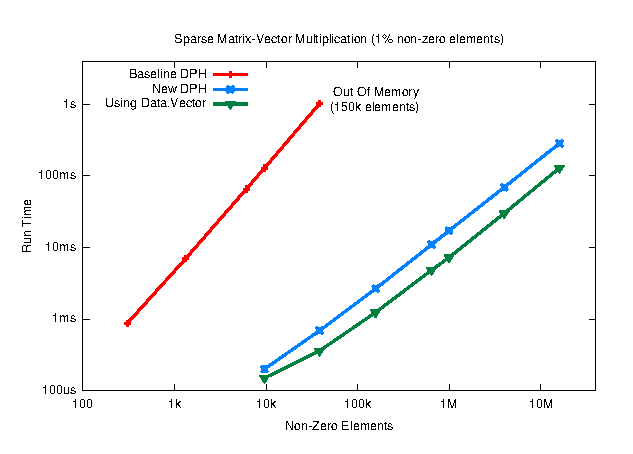
\includegraphics[scale=0.8]{data/smvm}
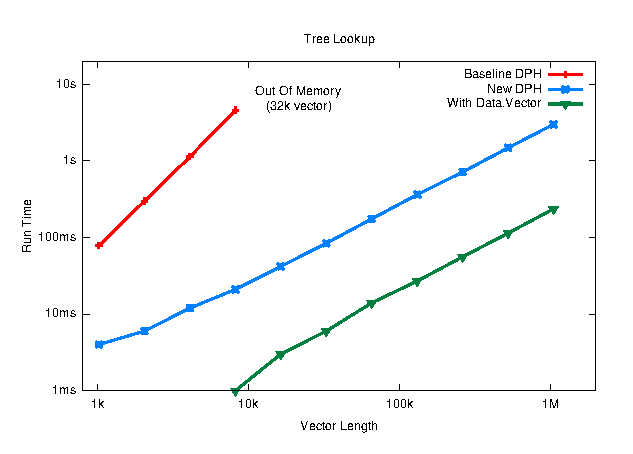
\includegraphics[scale=0.8]{data/indices}
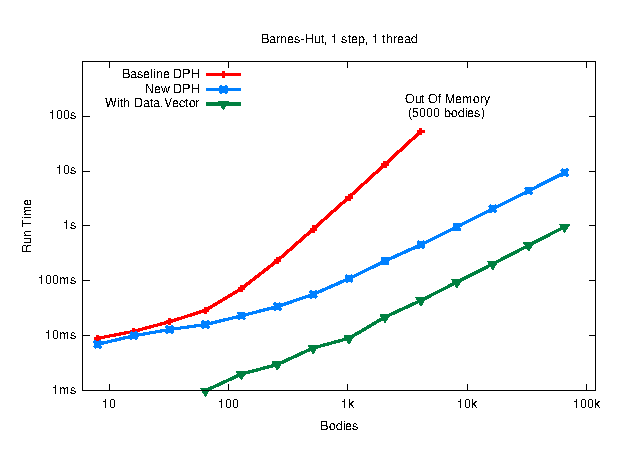
\includegraphics[scale=0.8]{data/nbody}
\caption{Benchmark Runtime Performance}
\label{figure:Benchmarks}
\end{figure}

When divide and conquer algorithms such as \mbox{Barnes-Hut} are vectorised, the resulting code increases the nesting level of the source array during the division phase (on the way down) and concatenates the result on the way back up. We refer to such algorithms as \emph{dynamically nested} for this reason. As discussed in \S\ref{section:ConcatUnconcat}, @concat@ normalises the array representation, so the program effectively switches between the old baseline representation and our new scattered representation as it runs.

\section{Related Work}
Approaches to the implementation of irregular parallelism roughly fall into two categories: thread-based implementations, like Manticore \cite{Fluet:2008:Manticore} or Ct \cite{ghuloum-etal:Ct}, and those based on flattening. Both have their advantages and drawbacks. With the former approach, scheduling, synchronisation, and granularity control are a concern, as well as a more restricted set of target architectures, though they do not suffer from the complexity problem described in this paper. However, the problem we describe is a fundamental issue for all flattening based approaches, and has been identified and discussed in several publications. 

The original first-order flattening transform and array representation shown in Figure~\ref{figure:OldArrayRepresentation} was introduced by Blelloch and Sabot in in \cite{Blelloch:compiling-collection-oriented-languages}. In this work the @replicate@ function is called @distribute@ when applied to scalars and @distribute-segment@ when applied to arrays. As a possible extension to the handling of conditionals they suggest operating on sparse segments instead of first eliminating gaps between them with the @pack@ operation. This idea is not elaborated further. The single example program they present (Quicksort) only uses @distribute@ and @pack@ on arrays of scalars, and thus does not suffer problems with asymptotic complexity. 

In \cite{Blelloch:vector-models} Blelloch proves that a subset of programs written with the scan-vector instruction set can be vectorised while preserving their asymptotic work and step complexity. Such programs must be both \emph{contained}, and not use indirect memory access, which is equivalent to disallowing functions to have free variables. Appendix C of the NESL manual \cite{Blelloch:nesl-3_1} gives the work complexity of vectorised programs, and states that the contents of free variables is copied across each iteration of the @apply-to-each@ (@map@) construct. Finally, in \cite{Blelloch:provable-type-and-space-efficient} the authors present a provably time and space efficient version of NESL, but the operational semantics is based around fine grained threads instead of SIMD style vectors. 

In \cite{Palmer:work-efficient-nested-data-parallelism}, Palmer et al.\ address the issue by disallowing partial applications and removing some of the problematic cases
using rewrite rules. For Haskell, ruling out partial applications to appear anywhere in a parallel context would be neither  desirable nor statically enforceable. The rewrite rules used do not fire if the offending index space transform is applied indirectly as part of another function. This is a general drawback of using rewrite rules, which can be acceptable if the rewriting only leads to a constant improvement, but not in our case, where the failure to identify problematic expressions results in asymptotically worse performance.

In \cite{Riely:flattening-improvement}, Riely and Prins solve this problem by using vectors of references, but at the time the article was written, there was no implementation, so they could not provide any experimental data as to the absolute performance. To the best of our knowledge, they have not published any further results on this approach. The suggested representation is similar to one of the states our representation can take on, for example, as a result of creating a nested vector by
collecting a number of different flat arrays in a nested one. However, the use of purely pointer based representations can lead to poor locality and complicates distribution and load balancing. It also increases garbage collection overhead, as every subarray must be traversed individually. In contrast, our approach aims at keeping the data representation as flat as possible, and only resorts to the partially flattened representation whenever the completely flat representation would lead to 
worse work complexity. 

\eject


% -----------------------------------------------------------------------------
\paragraph{Acknowledgements}
This work was supported in part by the Australian Research Council under grant number LP0989507.

\bibliographystyle{abbrvnat}
\bibliography{Main}


% -----------------------------------------------------------------------------
\appendix
%
\clearpage{}
% -----------------------------------------------------------------------------
\begin{figure}
\begin{small}
\begin{code}
-- Closures and closure arrays ------------------------
data (a :-> b) 
 = forall env. PA env 
 => Clo  (env -> a -> b) 
         (Int -> PData env -> PData a -> PData b) 
         env

data instance PData{s} (a :-> b)
 =  forall env. PA env
 => AClo  (env -> a -> b)
          (Int -> PData env -> PData a -> PData b)
          (PData{s} env)

-- Closure constructors -------------------------------
closure1 :: (a -> b) 
         -> (Int -> PA a -> PA b)
         -> (a :-> b)
closure1 fv fl
 = let  fl' n pdata
         = case fl n (PArray n pdata) of
                PA _ pdata' -> pdata'
   in   Clo  (\_env -> fv)
             (\n _env -> fl' n) ()

closure2 -> (a -> b -> c)
         -> (Int -> PA a -> PA b -> PA c)
         -> (a :-> b :-> c)
closure2 fv fl
 = let  fl' n pdata1 pdata2
         = case fl n (PA n pdata1) (PA n pdata2) of
                PA _ pdata' -> pdata'
        fv_1 _ xa   = Clo  fv fl' xa
        fl_1 _ _ xs = AClo fv fl' xs
   in   Clo fv_1 fl_1 ()

-- Closure and lifted closure application -------------
($:) :: (a :-> b) -> a -> b
($:) (Clo fv _fl env) x  = fv env x

($:^) :: PA (a :-> b) -> PA a -> PA b
PA n (AClo _fv fl envs) $:^ PA _ as 
        = PA n (fl n envs as)

-- Closure converted combinators ----------------------
indexPP :: PA a => PA a :-> Int :-> a
indexPP = closure2 PA.index PA.index_l

mapPP  :: (a :-> b) :-> PA a :-> PA b
mapPP   = closure2 mapPP_v mapPP_l
 where mapPP_v :: (a :-> b) -> PA a -> PA b
       mapPP_v f as
        =   replicatePA (lengthPA as) f $:^ as
       mapPP_l :: PA (a :-> b) -> PA (PA a) -> PA (PA b)
       mapPP_l fs ass
        =   unconcatPA ass 
        $   replicatesPA (takeLengths ass) fs
        $:^ concatPA ass

zipWithPP :: (a :-> b :-> c) 
          :-> PArray a  :-> PArray b :-> PArray c
zipWithPP   = closure3 zipWithPP_v zipWithPP_l
 where zipWithPP_v f xs ys
        =   replicatePA (lengthPA xs) f $:^ xs $:^ ys
       zipWithPP_l _ fs ass bss
        =   unconcatPA ass 
        $   replicatesPA (takeLengths ass) fs
        $:^ concatPA ass
        $:^ concatPA bss
\end{code}
\end{small}
\caption{Closure Converted Lifted Combinators.}
\label{figure:LiftedOperators}
\end{figure}

% -----------------------------------------------------------------------------
\begin{figure}
\begin{small}
\begin{code}
-- Vectorising Types -------------------------------------
Vt[T] :: Type -> Type
Vt[T1 -> T2] = Vt[T1] :-> Vt[T2] (functions)
Vt[ [:T:] ]  = Lt[T]             (parallel arrays)
Vt[ Int ]    = Int               (primitive scalar types)
Lt[T]        = PA Vt[T]


-- Vectorising Terms -------------------------------------
V[E] :: Term -> Term
V[k]       = k                   (literals)
V[f]       = f_PP                (f is bound at top level)
V[x]       = x                   (x is locally bound)
V[E1 E2]   = V[E1] $: V[E2]
V[\x -> E] = 
  Clo 
    { aenv  = (y_1, .., y_k)
    , aclov = \e x -> case e of (y_1, .., y_k) -> V[E]
    , aclol = \e x -> case e of ATup_k n' y_1 .. y_k -> L[e]n'}
  where
    {y_1, .., y_k} = free variables of \x -> E
V[if E1 then E2 else E3]
 = if V[E1] then V[E2] else V[E3]

Vtop[f x1 x2 .. = E1]            (toplevel binding)
 = let 
     fv   x1 x2 .. = V[E1]
     fl n x1 x2 .. = L[E1]n
     f_PP          = closure_N fv fl

-- Lifting Terms ----------------------------------------
L[E]n :: Term -> Term -> Term
L[k]n       = replicatePA n k     (literals)
L[f]n       = replicatePA n f_PP  (f is bound at top level)
L[x]n       = x                   (x is locally bound)
L[E1 E2]n   = L[E1]n $:^ L[E2]n
L[\x -> E]n = 
  AClo 
    { aenv  = ATup_k n y_1 .. y_k
    , aclov = \e x -> case e of (y_1, .., y_k) -> V[E]
    , aclol = \e x -> case e of ATup_k n' y_1 .. y_k -> L[e]n'}
  where
    {y_1, .., y_k} = free variables of \x -> E
L[if E1 then E2 else E3]n
 = let flags = L[E1]n
   in  combine flags (L[E2'] (countTrue  flags))
                     (L[E3'] (countFalse flags))
         with E2' = [{packPA fvs_i flags True  / fvs_i}]E2
              E3' = [{packPA fvs_i flags False / fvs_i}]E3

Ltop[f x1 x2 .. = E1]n            (toplevel binding)
 = let 
     fv   x1 x2 .. = V[E1]
     fl m x1 x2 .. = L[E1]m
     f_PP          = closure_N fv fl
\end{code}
\end{small}
\caption{The Vectorisation Transform}
\label{figure:VectorisationTransform}
\end{figure}



\clearpage{}
% -----------------------------------------------------------------------------
\section{Vectorisation of the retrieve function}
\label{section:VectorisationOfRetrieve}
The following is a derivation of the vectorised version of the @retrieve@ function discussed in \S2. 
\begin{small}
\begin{code}
 retrieve :: [:[:Char:]:] -> [:[:Int:]:] -> [:[:Char:]:]
 retrieve xss iss
   = zipWithP mapP (mapP indexP xss) iss
\end{code}
\end{small}
%
We first apply the vectorisation transform from Figure \ref{figure:VectorisationTransform}. This replaces application of library functions to their closure converted  (@*PP@) versions. The definitions of these functions are in Figure \ref{figure:LiftedOperators}.
\par
\begin{small}
\begin{code}
retrieve_v :: PA (PA a) -> PA (PA Int) -> PA (PA a))
retrieve_v xss iss
 = zipWithPP $: mapPP $: (mapPP $: indexPP $: xss) $: iss
\end{code}
\end{small}
%
We proceed by inlining the definitions of the library functions and simplify where appropriate. By doing this we will see how @replicates@ and @concat@ are introduced into the program. We start by  splitting out the partial application into its own binding to help the presentation.
%
\begin{small}
\begin{code}
 retrieve_v xss iss
  = let fs     = mapPP $: indexPP $: xss
    in  zipWithPP $: mapPP $: fs  $: iss
\end{code}
\end{small}
%
Inlining @zipWithPP@ and the first instance of @mapPP@ reveals that the closures for the worker functions are replicated. Inlining also introduces the lifted application operator (@$:^@). The definition of @mapPP@ is given in Figure \ref{figure:LiftedOperators}, and @zipWithPP@ is a simple extension.
%
\begin{small}
\begin{code}
 retrieve_v xss iss
  = let fs = (replicate (length xss) indexPP) $:^ xss
    in  (replicate (length iss) mapPP) $:^ fs $:^ iss
\end{code}
\end{small}
%
We now inline the lifted application operator (@$:^@). As @indexPP@ is partially applied, we end up with an explicit closure which captures the @xss@ array in its environment. In contrast, @mapPP@ has been fully applied, so the lifted application reduces to a direct application of the lifted map function @mapPP_l@. 
%
\begin{small}
\begin{code}
 retrieve_v xss iss
  = let fs = Clo index index_l xss
    in  mapPP_l fs iss
\end{code}
\end{small}
%
Inlining @mapPP_l@ reveals that segmented replicate is being applied to the closure representing the partial application of @indexP@ in the original program. Note that we are now using @replicatesPR@. The @*PR@ suffix indicates that the function works on the internal @PData@ type rather than the @PA@ wrapper.
%
\begin{small}
\begin{code}
 retrieve_v xss iss
  =   unconcat iss
  $   (let ns   = lengths $ takeSegd iss
           n    = sum ns
       in  PA n (replicatesPR ns 
                           (Clo index index_l xss)))
  $:^ concat iss
\end{code}
\end{small}
%
We now inline the @replicatesPR@ instance for closures. Performing segmented replicate on a closure produces an array closure where the environment has been replicated.
%
\begin{small}
\begin{code}
 retrieve_v xss@(PA _ xss') iss
  =   unconcat iss
  $   (let ns  = lengths $ takeSegd iss
           n   = sum ns
       in  PArray n (AClo index index_l 
                          (replicatesPR ns xss')))
  $:^ concat iss
\end{code}
\end{small}
%
Finally, we inline the remaining lifted application operator. This reveals that lifted indexing is being applied to our replicated tables array (@xss@). The vectorised function retrieves one element from each of the copies, then unconcatenates the result to produce the nesting structure of the original indices array (@iss@). 
%
\eject
\begin{small}
\begin{code}
retrieve_v xss@(PArray _ xss') iss@(PArray _ iss')
   = unconcat iss
   $ let ns  = lengths $ takeSegd iss
         n   = sum ns
     in  PArray n (indexlPR n (replicatesPR ns xss') 
                              (concatPR iss'))
\end{code}
\end{small}
%
We now consider what complexity bounds must be placed on the array operators so that the vectorised version of @retrieve@ has the same complexity as the original. The work complexity of the original is $O(length~ (concat~ \texttt{iss}))$. For the vectorised version to retain this complexity the operators @indexlPR@, @replicatesPR@ and @concatPR@ must all be linear in the length of their results. Since @retrieve@ is polymorphic in the element type @a@, the array operators must have this complexity for possible element types. This includes arrays of arbitrary nesting depth.


\clearpage{}
% -----------------------------------------------------------------------------
\section{Vectorisation of the retsum function}
The @retsum@ function indexes several shared arrays, and adds the retrieved value to the sum of the array it came from. This has a similar structure to @retrieve@ from the previous section.
%
\begin{small}
\begin{code}
 retsum :: [:[:Int:]:] -> [:[:Int:]:] -> [:[:Int:]:]
 retsum xss iss
  = zipWithP mapP 
            (mapP (\xs i. indexP xs i + sumP xs) xss) iss
\end{code}
\end{small}
%
Applying the vectorisation transform yields:
%
\begin{small}
\begin{code}
 retsum_v xss iss
  = let fv ys j     = index ys j + sum ys
        fl c yss js = add_l c (index_l c yss js) 
                              (sum_l   c yss)
        fPP         = closure2 fv fl
    in  zipWithPP $: mapPP $: (mapPP $: fPP $: xss) $: iss
\end{code}
\end{small}
%
Shift partial application into own binding and inline @zipWithPP@
%
\begin{small}
\begin{code}
 retsum_v xss iss
  = let c            = length iss
        fv ys j      = index ys j P.+ sum ys
        fl c' yss js = add_l c' (index_l c' yss js) 
                                (sum_l   c' yss)
        fPP     = closure2 fv fl
        gs      = mapPP $: fPP $: xss
    in  replicate c mapPP $:^ gs $:^ iss
\end{code}
\end{small}
%
Inline @closure2@ and @replicates@ instances.
%
\begin{small}
\begin{code}
 retsum_v _xss@(PA _ xss') iss
  = let c            = length iss
        fv ys j      = index ys j P.+ sum ys
        fl c' yss js = add_l c' (index_l c' yss js) 
                                (sum_l   c' yss)

        fl' n pdata1 pdata2
         = case fl n (PA n pdata1) (PA n pdata2) of
            PA _ pdata' -> pdata'
        
        fl_1 _ _ xs = AClo fv fl' xs
        gs          = PA c (fl_1 c (replicatePR c ()) xss')
    in  replicate c mapPP $:^ gs $:^ iss
\end{code}
\end{small}
%
Inline @fl_1@, @mapPP@, and @replicate@ on closures.
%
\begin{small}
\begin{code}
 retsum_v _xss@(PA _ xss') iss
  = let fv ys j = index ys j P.+ sum ys
        fl c' yss js = add_l c' (index_l c' yss js) 
                                (sum_l   c' yss)

        fl' n pdata1 pdata2
         = case fl n (PA n pdata1) (PA n pdata2) of
            PA _ pdata' -> pdata'

    in  unconcat iss
         $ (let ns = lengths iss
                n  = sum ns
            in  PA n (AClo fv fl' (replicatesPR ns xss')))
         $:^ concat iss
\end{code}
\end{small}
%
Inline lifted applications.
%
\begin{small}
\begin{code}
 retsum_v xss iss
  = let fl c' yss js = add_l c' (index_l c' yss js) 
                                (sum_l   c' yss) 
    in  unconcat iss
         $ (let ns = lengths iss
                n  = sum ns
            in  fl n (replicates ns xss) (concat iss))
\end{code}
\end{small}

\eject
\noindent
Inline @fl@ and float bindings.
%
\begin{small}
\begin{code}
 retsum_v xss iss
  = let  ns      = lengths iss
         n       = sum ns
         yss'    = replicates ns xss
    in   unconcat iss 
          $ add_l n (index_l n yss' (concat iss)) 
                    (sum_l   n yss')
\end{code}
\end{small}

% -----------------------------------------------------------------------------
\section{Vectorisation of the furthest function}
The @furthest@ function takes an array of points and computes the maximum distance between any pair. 

\begin{small}
\begin{code}
 furthest :: [:(Float, Float):] -> Float
 furthest ps = maxP (mapP (\p. maxP (mapP (dist p) ps)) ps)

 dist :: (Float, Float) -> (Float, Float) -> Float
\end{code}
\end{small}
%
Applying the vectorisation transform yields:
%
\begin{small}
\begin{code}
 furthest_v :: PA Int -> Int
 furthest_v xs
  = let  fv :: Int -> Int
         fv       = unused
        
         fl :: Int -> PA Int -> PA Int
         fl c ys  =    replicate c maxPP 
                  $:^ (replicate c mapPP 
                         $:^ (replicate c distPP $:^ ys) 
                         $:^  replicate c xs)

         fPP      :: Int :-> Int
         fPP      = closure1 fv fl
        
   in    maxPP $: (mapPP $: fPP $: xs)  
\end{code}
\end{small}
%
Inline @maxPP@, @fPP@ and last occurrence of @mapPP@.
%
\begin{small}
\begin{code}
 furthest_v xs
  = let fl c ys  = max_l c 
                 $ replicate c mapPP 
                     $:^ (replicate c distPP $:^ ys)
                     $:^ replicate c xs
  in    max (fl (length xs) xs)
\end{code}
\end{small}
%
Inline inner @mapPP@.
%
\begin{small}
\begin{code}
 furthest_v xs
  = let fl c ys  
         = let xss'     = replicate c xs
           in  max_l c 
                $   unconcat xss'
                $   replicates (lengths xss') 
                     ((replicate c distPP) $:^ ys)
                $:^ concat xss'
    in  max (fl (length xs) xs)
\end{code}
\end{small}
%
Float bindings.
%
\begin{small}
\begin{code}
 furthest_v xs
  = max (let c    = length xs
             xss' = replicate c xs
         in  max_l c 
              $   unconcat xss'
              $   replicates (lengths xss') 
                   ((replicate c distPP) $:^ xs)
              $:^ concat xss')
\end{code}
\end{small}

\eject
\noindent
Inline @distPP@ closure.
%
\begin{small}
\begin{code}
 furthest_v xs
  = let c       = length xs
        xss'    = replicate c xs
        ns      = lengths xss'

        fl' n pdata1 pdata2
         = case dist_l n (PA n pdata1) (PA n pdata2) of
            PA _ pdata' -> pdata'

        fv_1 _ xa    = Clo  dist fl' xa
        fl_1 _ _ xs' = AClo dist fl' xs'
        clo          = Clo fv_1 fl_1 ()
    in  max $   max_l c 
            $   unconcat xss'
            $   replicates ns ((replicate c clo) $:^ xs)
            $:^ concat xss'
\end{code}
\end{small}
%
Inline @clo@
%
\begin{small}
\begin{code}
 furthest_v xs@(PA _ xs')
  = let c       = length xs
        xss'    = replicate c xs
        ns      = lengths xss'

        fl' n pdata1 pdata2
         = case dist_l n (PA n pdata1) (PA n pdata2) of
            PA _ pdata' -> pdata'
        
    in  max $   max_l c 
            $   unconcat xss'
            $   replicates ns (PA c (AClo dist fl' xs'))
            $:^ concat xss'
\end{code}
\end{small}
%
Inline @replicates@ and final lifted application.
%
\begin{small}
\begin{code}
 furthest_v xs@(PAy _ xs')
  = let c       = length xs
        xss'    = replicate c xs
        ns      = lengths xss'

        fl' n pdata1 pdata2
         = case dist_l n (PA n pdata1) (PA n pdata2) of
            PA _ pdata' -> pdata'
                
    in  max $ max_l c 
            $ unconcat xss'              
            $ (case concat xss' of
                PA _ xssd
                 -> PA  (sum ns) 
                  $ fl' (sum ns) (replicatesPR ns xs') xssd)
\end{code}
\end{small}
%
Inline @fl'@ and simplify.
%
\begin{small}
\begin{code}
 furthest_v xs
  = let  c    = length xs
         xss' = replicate c xs
         ns   = lengths xss'     
    in   max  $ max_l c 
              $ unconcat xss'              
              $ dist_l (U.sum ns) 
                       (replicates ns xs) (concat xss')
\end{code}
\end{small}
%
Note that if @c@ is the length of @xs@ all $O(@c@^2)$ distances will be computed by @dist_l@ before @max@ and @max_l@ determine the greatest one. When run sequentially, the source function would use space linear in the length of @xs@, but the vectorised version uses space quadratic in the length of @xs@. This exposes the maximal amount of parallelism, at the cost of increased space complexity to hold the intermediate values.


\eject
% -----------------------------------------------------------------------------
\section{Segment Descriptor Culling Functions}


\begin{small}
\begin{code}
-- | Drop physical segments in a SSegd that are unrechable
--   from the segmap, and rewrite the segmap to match.
cullOnSegmap :: Vector Int -> SSegd -> (Vector Int, SSegd)
cullOnSegmap segmap (SSegd sources starts (Segd lengths _))
 = (segmap', ssegd')
 where
    (used_flags, used_map) 
     = makeCullMap (length sources) segmap 

    -- Use the used_map to rewrite the segmap to point to
    -- the corresponding psegs in the result.
    --  Example:   segmap:  [0 1 1 3 5 5 6 6]
    --           used_map:  [0 1 -1 2 -1 3 4]
    --            segmap':  [0 1 1 2 3 3 4 4]
    segmap'   = map (used_map !) segmap

    -- Drop unreachable psegs entries from the SSegd.
    starts'   = pack starts  used_flags
    sources'  = pack sources used_flags
    lengths'  = pack lengths used_flags

    ssegd'    = SSegd sources' starts' 
              $ segdOfLengths lengths'


-- | Drop data chunks in a PDatas that are unreachable
--   from the SSegd, and rewrite the SSegd to match.
cullOnSSegd :: PR a => SSegd -> PDatas a -> (SSegd, PDatas a)
cullOnSSegd (SSegd sources starts segd) pdatas
 = (ssegd', pdatas')
 where
    (used_flags, used_map)
     = makeCullMap (lengthdPR pdatas) sources

    -- Rebuild the SSegd.
    sources' = map (used_map !) sources
    ssegd'   = SSegd sources' starts segd

    -- Drop unreachable chunks from the PDatas.
    pdatas'  = packdPR pdatas used_flags 


makeCullMap:: Int -> Vector Int ->(Vector Bool, Vector Int)
makeCullMap total used
 = (flags, used_map)
 where 
    -- Make an array of flags signalling whether each
    -- element is used or not.
    -- Example: used:  [0 1 1 3 5 5 6 6]
    --       => flags: [T T F T F T T]
    flags
     = backpermuteDft total (const False)
     $ zip used 
           (replicate (length used) True)

    -- Make a set of used indices.
    --  Example: flags:    [T T F T F T T]
    --       =>  uset_set: [0 1 3 5 6]
    used_set
     = pack (enumFromN 0 (length flags)) flags

    -- Make am array that maps used elements in the source
    -- array onto elements in the result array.
    -- If a particular element isn't used this maps to -1.
    -- Example: used_set:  [0 1 3 5 6]
    --          used_map:  [0 1 -1 2 -1 3 4]
    used_map
     = backpermuteDft total (const (-1 :: Int))
     $ zip used_set 
           (enumFromN 0 (length used_set))

\end{code}
\end{small}


% -----------------------------------------------------------------------------
\section{Virtual Shared Indexing}

The following @indexvsPR@ function implements virtual shared indexing for nested arrays and is described in \S5.1 of the main paper.

\begin{small}
\begin{code}
instance PR a => PR (PA a) where
 indexvsPR (PNesteds pdatas) vsegd1 srcixs
  = PNested vsegd' pdatas'
  where 
    -- O(length segixs)
    (segLengths, segStarts, segBlocks)
     = unzip3
     $ map (\(ix1, ix2) -> 
        let -- Index into the outer array.
            ssegd1  = ssegd   vsegd1
            psegid1 = segmap  vsegd1 ! ix1
            source1 = sources ssegd1 ! psegid1
            start1  = starts  ssegd1 ! psegid1

            -- Index into the inner arrays.
            arr2    = pdatas  ! source1
            vsegd2  = vsegd   arr2
            ssegd2  = ssegd   vsegd2
            segd2   = segd    ssegd2
            psegid2 = segmap  vsegd2 ! (start1 + ix2)
            source2 = sources ssegd2 ! psegid2
            start2  = starts  ssegd2 ! psegid2
            length2 = lengths segd2  ! psegid2
            block2  = pdata   arr2 `indexdPR` source2
        in  (length2, start2, block2))
     $ srcixs
        
    -- O(length segixs)
    vsegd'  = promoteSSegd
            $ SSegd (enumFromN 0 (length srcixs)) 
                    segStarts
            $ segdOfLengths segLengths

    -- O(length flats) = O(length segixs)
    pdatas' = concatdPR
            $ map singletondPR segBlocks
\end{code}
\end{small}

\vfill

\eject
% -----------------------------------------------------------------------------
\section{Virtual Shared Extraction}
The following @extractvsPR@ function implements virtual shared extraction for nested arrays and is described in \S5.1 of the main paper.

\begin{small}
\begin{code}
instance PR a => PR (PA a) where
 extractvsPR (PNesteds pdatas) vsegd1 
  = PNested vsegd' pdatas_culled
  where
    ssegd1      = demoteVSegd vsegd1
    segLengths  = lengths $ segd ssegd1
    segSources  = sources ssegd1

    -- Get the array id for each segment in the result.
    src_sources = replicates segLengths segSources
        
    -- Gather up the segmaps from each source array.
    segmaps    = PInts $ map  (segmap . vsegd)  pdatas
    sourcess_v = map (sources . ssegd . vsegd)  pdatas
    startss_v  = map (starts  . ssegd . vsegd)  pdatas
    lengthss_v = map (lengths.segd.ssegd.vsegd) pdatas

    -- Get the psegid to use for each segment in the
    -- result, relative to the source arrays.
    PInt src_psegids = extractvsPR segmaps vsegd1

    -- Because all the flat arrays go into the result, 
    -- we need to adjust the source ids from the
    -- original arrays.
    psrcoffset = prescanl (+) 0 
               $ map (lengthdPR . pnestedPData) pdatas

    -- Get the block id for each segment in the result.
    dst_sources 
     = zipWith (\src pseg -> (sourcess_v ! src) ! pseg 
                          +   psrcoffset ! src)
               src_sources src_psegids
        
    -- Get the start index for each segment in its block.
    dst_starts 
     = zipWith (\src pseg -> (startss_v ! src) ! pseg)
               src_sources src_psegids

    -- Get the length of each segment in the result.
    dst_lengths 
     = zipWith (\src pseg -> (lengthss_v ! src) ! pseg)
               src_sources src_psegids

    -- Build the SSegd for the result.
    -- This references all data blocks in the source.
    ssegd_all   = SSegd dst_sources dst_starts
                $ segdOfLengths dst_lengths

    -- Collect up all blocks from the source.
    pdatas_all  = concatdPR $ map pnestedPData pdatas

    -- Cull the blocks from the source array so the
    -- SSegd only references the ones needed in the
    -- result.
    (ssegd_culled, pdatas_culled)
                = cullOnSSegd ssegd_all pdatas_all

    -- Build the final VSegd
    vsegd'      = promoteSSegd ssegd_culled   
\end{code}
\end{small}


% -----------------------------------------------------------------------------
\clearpage{}
\section{Barnes-Hut Kernel}
This is the kernel of the Barnes-Hut benchmark described in \S7 of the main paper.
\begin{small}
\begin{code}
-- A point with some mass.
data MassPoint   = MP  Double Double Double
--                       X      Y     mass

-- Acceleration vector.
type Accel       = (Double, Double)

-- Bounding box for points.
data BoundingBox = Box Double Double Double Double

-- The Barnes-Hut Quad-Tree
data BHTree
    = BHT Double          -- Size of box.
          Double          -- Centroid X.
          Double          -- Centroid Y.
          Double          -- Centroid mass.
          [:BHTree:]      -- Children.

-- | Given a bounding box containing all the points,
--   calculate their accelerations.
calcAccelsWithBox
    :: Double             -- Simulation smoothing param.
    -> BoundingBox -> [:MassPoint:] -> [:Accel:]

calcAccelsWithBox epsilon box points
 = [: calcAccel epsilon m tree | m <- points :]
 where tree = buildTree box points

-- | Build the Barnes-Hut quadtree tree.
buildTree :: BoundingBox -> [:MassPoint:] -> BHTree
buildTree bb points
 | lengthP points <= 1      = BHT s x y m emptyP
 | otherwise                = BHT s x y m subTrees
 where  MP x y m            = calcCentroid points
        (boxes, splitPnts)  = splitPoints bb points
        subTrees               
             = [: buildTree bb' ps 
                  | (bb', ps) <- zipP boxes splitPnts:]
  
        Box llx lly rux ruy = bb
        sx   = rux - llx
        sy   = ruy - lly
        s    = if sx < sy then sx else sy

-- | Split points according to their locations in
--   the quadrants.
splitPoints
        :: BoundingBox
        -> [: MassPoint :]
        -> ([:BoundingBox:], [:[: MassPoint :]:])

splitPoints b@(Box llx lly rux  ruy) points 
  | noOfPoints <= 1 = (singletonP b, singletonP points)
  | otherwise         
  = unzipP [: (b,p) | (b,p) <- zipP boxes splitPars
                    , lengthP p > 0:]
  where noOfPoints  = lengthP points
        lls         = [: p | p <- points, inBox b1 p :]
        lus         = [: p | p <- points, inBox b2 p :]
        rus         = [: p | p <- points, inBox b3 p :]
        rls         = [: p | p <- points, inBox b4 p :]
        b1          = Box llx  lly  midx midy
        b2          = Box llx  midy midx  ruy
        b3          = Box midx midy rux   ruy
        b4          = Box midx lly  rux  midy
        boxes       = [:b1,  b2,  b3,  b4:] 
        splitPars   = [:lls, lus, rus, rls:]
        (midx,  midy) = ((llx + rux) / 2.0, (lly + ruy) / 2.0) 
\end{code}
\end{small}

\eject
\begin{small}
\begin{code}
-- | Check if point is in box.
--   (excluding left and lower border)
inBox :: BoundingBox -> MassPoint -> Bool
inBox (Box llx  lly rux  ruy) (MP px  py  _) 
 = (px > llx) && (px <= rux) && (py > lly) && (py <= ruy)


-- | Calculate the centroid of some points.
calcCentroid:: [:MassPoint:] -> MassPoint
calcCentroid mpts 
 = MP  (sumP xs / mass) (sumP ys / mass) mass
 where 
   mass     = sumP   [:m              | MP _ _ m  <- mpts:]
   (xs, ys) = unzipP [:(m * x, m * y) | MP x y m  <- mpts:]   


-- | Calculate the acceleration of a point due to the
--    points in the given tree.
calcAccel :: Double 
          -> MassPoint -> BHTree -> (Double, Double)

calcAccel epsilon point (BHT s x y m subtrees)
        | lengthP subtrees == 0
        = accel epsilon point (MP x y m)

        | isFar mpt s x y 
        = accel epsilon point (MP x y m)

        | otherwise
        = let (xs, ys) 
               = unzipP [: calcAccel epsilon point st 
                        |  st <- subtrees :]
          in  (sumP xs, sumP ys)


-- | Calculate the acceleration between points.
accel   :: Double    -- Smoothing parameter.
        -> MassPoint -- The point being accelerated.
        -> MassPoint -- Neighbouring point.
        -> Accel

accel epsilon (MP x1 y1 _) (MP x2 y2 m)  
 = (aabs * dx / r , aabs * dy / r)  
 where  rsqr = (dx * dx) + (dy * dy) + epsilon * epsilon
        r    = sqrt rsqr 
        dx   = x1 - x2 
        dy   = y1 - y2 
        aabs = m  / rsqr 


-- | If the point is far from a box in the tree then we
--   can use its centroid as an approximation of all the
--   points in the corresponding branch.
isFar   :: MassPoint  -- Point being accelerated.
        -> Double     -- Size of box.
        -> Double     -- X pos of centroid.
        -> Double     -- Y pos of centroid.
        -> Bool

isFar (MP x1 y1 m) s x2 y2 
 = let  dx      = x2 - x1
        dy      = y2 - y1
        dist    = sqrt (dx * dx + dy * dy)
   in   (s / dist) < 1
\end{code}
\end{small}

% 
\clearpage{}
\section{Notes and unused text}

% -----------------------------------------------------------------------------
\subsection{
        \cite{Blelloch:compiling-collection-oriented-languages}
        Blelloch 1989: Compiling Collection Oriented Languages}
\begin{itemize}
\item	Source language is Paralation LISP, not NESL yet.
\item	Vectorisation is mapping of data structures as well as transformation of source code.
\item	Describes plain segment descriptor representation. Array is data elements plus lengths of segments.
\item	Section 5.2.2 explains how free variables of an @elwise@ should be copied across all elements of the @elwise@. Like \emph{scalar extension} from APL, but any value will be copied, not just scalars.
\item	Replicate function is called @distrubute@ (for scalars) and @distribute-segment@ (for arrays) instead. \emph{``If the value is a field, a @distribute-segment@ operation is inserted that creates a nested field with the original field in each element''}.
\item	Has only one example program, QuickSort.
\item	The single QuickSort example given only uses plain @distribute@ on a scalar, not @distribute-segment@ on arrays. Quicksort needs to distribute the pivot to each array element to do the comparision.
\item	With QuickSort, the level of nesting increases with every step in the recursion.
\item	Mentions trade-offs with packing sparse segments. When a variable is free in both alternatives of an if-then-else expression, may want alternatives to operate on the sparse segments instead of packing down to just the ones relative to each alternative.
\end{itemize}


% -----------------------------------------------------------------------------
\subsection{Blelloch 1990: Vector models for parallel computing}
\begin{itemize}
\item	Riely1995 states that this text proves a that the high-level step/work metric of a program accurately reflects its cost on a VRAM, but only for the class of expressions with no free variables.
\item   Lifting of functions to vector form is referred to as \emph{code replicating}. 
\end{itemize}


% -----------------------------------------------------------------------------
\subsection{
        \cite{Prins:transformation-vector-operations}
        Prins 1993: Transforming High-Level Data-Parallel Programs into Vector Operations }

\begin{itemize}
\item	Mentions replicate/index problem in Section 4.5. Says that shared array should not be replicated, but does not give a transformation for it, or discuss how this optimisation should be applied in the general case. \ben{Problem is that user defined functions can perform indexing internally, so rewrite rules that operate on replicate/index pairs won't apply universally.}
\item	Function values must be fully parameterised, no partial application.
\item	Presents vectorisation as a formal program transformation, instead of as English Prose as in Blelloch 1989.
\item	Replicates variables free in iterator expressions, in rule (R2d) of Section 3.
\end{itemize}


% -----------------------------------------------------------------------------
\subsection{Hill 1993: Vectorising a non-strict data parallel functional language}


% -----------------------------------------------------------------------------
\subsection{
        \cite{Blelloch:implementation-portable}
        Blelloch 1994: Implementation of a Portable Nested Data-Parallel Language}
\begin{itemize}
\item 	Discusses NESL as an interpreter that issues VCODE instructions on segmented arrays.
\item 	Benchmarks paper. Gives brief overview of NESL then presents example programs.
\item 	Says one of the main overheads is the fine granularity of instructions issued by the interpreter.
\end{itemize}

% -----------------------------------------------------------------------------
\subsection{Riely 1994: Compilation of Nested Parallel Programs: Soundness and Efficiency}


% -----------------------------------------------------------------------------
\subsection{Blelloch 1995: NESL A Nested Data Parallel Language}
\begin{itemize}
\item	Comes in several versions as CMU technical reports dated Jan 1992, April 1993, September 1995.
\item 	Both equations given in Section 1.5 to calculate the complexity of apply-to-each have exceptions. 
\item	First exception introduces the idea of a \emph{contained} function. Non-contained functions have a different depth complexity in an apply-to-each. 
\item	Second exception is the replicate problem. States that the free variables in an apply-to-each are copied across each iteration.
\end{itemize}


% ----------------------------------------------------------------------------
\subsection{
        \cite{Riley:provably-correct-vectorisation}
        Riely 1995: Provably Correct Vectorisation of Nested-Parallel Programs}
\begin{itemize}
\item	Equivalence of programs includes the asymptotic efficiency.

\item	Introduces idea of contained functions.

\item	States that the discussion of the handling of free variables is the main contribution of the paper.

\item	Describes three alternative semantics: \emph{ideal}, where the step complexity of an iterator is just the maximum of all steps taken by the iterator; \emph{construct-parameters}, where free variables are copied across each iteration, as used by NESL; \emph{construct-results}, middle ground between the two that relies on static analysis, as used by Proteus as in \cite{Palmer:work-efficient-nested-data-parallelism}.

\item	States that \emph{ideal} semantics forces a reference-based implementation of sequences, with the necessity of unbounded contention on a CREW PRAM. \ben{DPH shows that we don't actually need a reference-based implementation}.  

\item	Gives complexity bounds on the array primitives. The function @dist(n, A)@ (replicate) must have work proportional to @n@. The functions @rstr@ and @comb@ (pack and combine) must have work proportional to the length of their first arguments. ``Note that these restrictions point to a reference based implementation''. 

\item	Says that we cannot implement the ideal semantics in a bounded-CREW machine, and that one solution is to copy free variables of array comprehensions across all iterations. \ben{This is over pessimistic. We need concurrent reads proportional to the number of threads, not the number of array elements. In a multicore setting, the number of threads is much smaller than the number of array elements. In a machine with a hierarchical cache, access to shared data implicitly copies it out to thread-local caches.}

\item	Gives complexity bounds on @pack@ and @combine@ to achieve the ideal semantics.

\item	The construct-result semantics bans the use of user defined projection functions.

\item	Uses ``lifted'' terminology to refer to version of functions that work on arrays.
\end{itemize}


% -----------------------------------------------------------------------------
\subsection{
        \cite{Palmer:work-efficient-nested-data-parallelism}
        Palmer 1995: Work Efficient Nested Data Parallelism (Proteus) }
\begin{itemize}
\item	Explicitly says that vectorisation has a problem with un-nessesary replication with index operations.

\item	Implements randomised indexing to reduce concurrent reads.

\item	Says that NESL provides many primitives that, in parallel, select values from sequences in common access patterns. Using these functions interferes with function modularity, because programmer needs to move single operations from inside functions to outside, to work on the aggregate. Need to specialise each function containing indexing to every call pattern, depending on what shared structure it is indexing.

\item	No partial application. Functions must be fully applied.

\item	\ben{When vectorising Haskell, cannot use this approach because the thunk passed into a higher order function may have a closure containing a shared array. Cannot vectorise functions based on whether their arguments are shared because this information isn't visible. Even if it was, would need to specialise functions for every call pattern.}

\item	Discusses using a rewrite rule to transform \\ @index^ (rep n arr) ixs@ into @indexs arr ixs@. \ben{Point out problem with rewrite rule. If the nested array to be indexed is the result of an arbitrary function call, then the rule will not fire. In the following code, the call to the known function @f@ prevents using this transform when vectorising @thing@.}

\begin{code}
xs  = [...]
thing f arr ixs = mapP (! (f arr)) ixs
main            = thing length xs ...
\end{code}

\item	Has hierarchical indices and copies the top level of the tree to reduce the number of concurrent reads. Expect this is not needed for current architectures.

\item	Tags array variables that are only used as the source of an indexing operation with a new primitive @only_indexed@. Says to use an (un-described) static analysis to propagate @only_indexed@ across function call boundaries and throughout the program. The primitive @only_indexed@ is at the value level, not the type level. It seems one should use a fixpoint process to propagate it, instead of unification of types. This process won't work with higher order functions. Will fix the replication problem for some specific examples, but is not a general solution for higher-order programs.
\end{itemize}


% -----------------------------------------------------------------------------
\subsection{Palmer 1995: Piecewise Execution of Nested Data-Parallel Programs}


% -----------------------------------------------------------------------------
\subsection{Blelloch 1996: A Provable Time and Space Efficient Implementation of NESL}


% -----------------------------------------------------------------------------
\subsection{Riely 2000: Flattening is an Improvement}
\begin{itemize}
\item   Containment is not sufficient to guarantee that flattening results in weak improvement.
\end{itemize}



% ---------------------------------------------------------------------------
\subsection{Leshchinskiy 2002: Costing nested array codes}

% ----------------------------------------------------------------------------
\subsection{Spoonhower 2008: Space Profiling for Parallel Functional Programs}



\clearpage{}
% -- QuickHull ----------------------------------------------------------------
\subsection{QuickHull}
\begin{itemize}
\item	Example of a program that does not suffer the replicate problem. No free variables are captured and replicated in the closures.
\end{itemize}

\begin{small}
\begin{code}
split :: [:Point:] -> Line -> [:Point:]
split points line@(p1, p2)
 | lengthP packed == 0 = [:p1:]
 | otherwise
 = concatP [: split packed ends 
            | ends <- [:(p1, pm), (pm, p2):] :]
 where
  cross  = [: distance p line | p <- points :]
  packed = [: p | (p,c) <- zipP points cross, c > 0.0 :]
  pm     = points !: maxIndexP cross

distance :: Point -> Line -> Double
distance (xo, yo) ((x1, y1), (x2, y2))
 = (x1-xo) * (y2 - yo) - (y1 - yo) * (x2 - xo)
\end{code}
\end{small}


\clearpage{}
% -----------------------------------------------------------------------------
\section{The Trouble with Index Space Transforms}

Vectorisation has three main components: the transform that rewrites the user program to use primitive parallel array operators, the implementation of those operators, and the array representation itself. Although we sometimes refer to just the program transform as ``vectorisation'', the three components are inseparable as the design of each has profound effects on the others. Figure \ref{figure:VectorisationTransform} shows the complete vectorisation transform, though we will introduce it in stages throughout this paper. Figure \ref{figure:UserVisibleArrayOperators} shows some representative user-visible array operators, while Figure \ref{figure:OldArrayRepresentation} gives our old array representation and signatures for some parallel primitives. We will improve over these in the coming sections.

The operators in Figure \ref{figure:OldArrayRepresentation} are all \emph{index space transforms}. They change the mapping of array indices to array elements, but do not create new element values. The fact that vectorisation introduces such transforms is to be expected, as its purpose is to provide a mapping between the singular bulk array operations that the user writes, and the many parallel processors of the underlying machine. Vectorisation is a process of ``rearrangement'', rather than the definition of new values.

Returning to the @gather@ example from \S\ref{section:Introduction}, the vectorised version has the wrong complexity because the index space transform @replicate@ was implemented by physically copying data. This was a consequence of the representation of nested arrays used in NESL, and inherited by DPH. For example, replicating the array @[1 2 3 4 5]@ four times yields a value 
of type @PA (PA Int)@, which is represented thus:

\begin{small}
\begin{code}
  [[1 2 3 4 5] [1 2 3 4 5] [1 2 3 4 5] [1 2 3 4 5]]
 ----------------------------------------------- (ARR0)
  PA 4 (PNested
   (Segd lengths: [5 5 5 5] indices: [0 5 10 15]
           elems: 20)
   (PInt [1 2 3 4 5 1 2 3 4 5 1 2 3 4 5 1 2 3 4 5]))
\end{code}
\end{small}

We have shown the \emph{logical value} of the array above the line, and its \emph{physical representation} below. The representation is determined by the data type declararations in Figure~\ref{figure:OldArrayRepresentation}.  Every @PA@ value is built with an outer @PArray@ constructor,
with the payload in the @pdata@ field of type @PData (PA a)@.  The @lengths@ field gives the lengths of the inner arrays, also known as \emph{segments}, while the @indices@ field gives the starting index of each segment in the @PData@ array. A @Vector@ is a primitive flat array of elements. The @lengths@ and @indices@ are bundled up into the \emph{segment descriptor} @Segd@. Arrays of greater nesting depth are created by adding more @Segd@ layers on top. We will give an example of this in \S\ref{section:Replicate}.

Nested arrays are given this representation for two reasons: so all the element data lie contiguously in a single flat array, and so the nested array can be concatenated simply by discarding the segment descriptor. Storing the element data in a single flat array allows us to process it with the fast vector operations supported by the underlying hardware. Concatenation is used when vectorising higher-order functions, and is the core feature of the \emph{flattening nested parallelism} approach. We will discuss this further in \S\ref{section:ConcatUnconcat}. Unfortunately, although the array representation has these two fundamental properties, it cannot be used to represent index space transforms such as replication without copying data. This shortfall, in turn, can break the complexity of the vectorised programs. This brings us to the question of why we need such transforms in the first place.


% -----------------------------------------------------------------------------
\subsection{Replicate Operations Broadcast Shared Values}
On an abstract level, the role of @replicate@ is to \emph{broadcast} a shared value to all processors in the machine. For example, suppose our machine model supports lifted addition as a parallel primitive:
\begin{code}
  add_l :: Int -> PA Int -> PA Int -> PA Int
\end{code}

This function takes two arrays of the same length, adds corresponding elements together, and produces an array of results. The first argument is the \emph{lifting context}, which provides the length of the argument and result arrays, and represents the maximum number of parallel tasks. Suppose we wish to evaluate the following:
\begin{code}
  add_l 4 [1 2 3 4] [6 7 8 9]
\end{code}

Ignoring practical issues with small grain size, to evaluate this expression on a four processor machine we could send one pair of elements to each processor. Suppose instead we want to add the value @10@ to every element of the second array. We can also do this with @add_l@, provided we send the shared value to each processor. This is the job of @replicate@:
\begin{code}
  add_l 4 (replicate 4 10) [6 7 8 9]
\end{code}

The type of @add_l@ suggests a machine model where the processors are physically separate. Each pair of integers is added individually, and the addition of each pair does not affect another. With this model, replicating shared values by physically copying them makes sense. For example, the ``processors'' might be the ALU slices that implement the SIMD-ways in a vector machine, and @replicate@ would fill a vector register with copies of a the same scalar value. However, if the additions were instead performed individually on a shared-memory multicore machine, then replicating a shared value by physically copying would just waste work and space.

Instead, want each processor to read a single instance of the shared value. On the physical level, the cache hardware will then make as many additional copies as it sees fit, though we assume that these additional copies are not visible from the programming model of our implementation language. Adding a shared value to all the elements of an array is embodied by the following operator:
\begin{code}
  add_s :: Int -> Int -> PA Int -> PA Int
\end{code}

In contrast to @add_l@, the first array parameter has been replaced by a single scalar which will be shared during the computation. We highlight the distinction between @add_l@ and @add_s@ because the vectorisation transform itself only introduces the former. Given a user-defined function such as:
\begin{code}
 z           = 5
 f x y       = add z (add x y)
\end{code}

\noindent
The vectoriser creates a lifted version of @f@ as follows:
\begin{code}
 z           = 5
 f_l c xs ys = add_l c (replicate c z) (add_l xs ys)
\end{code}

The lifted version @f_l@ performs the same operation as @f@, except that it works on multiple values at the same time, in parallel. The vectoriser \emph{lifts} each of the parameters of the original function to \emph{vector space} (it makes them arrays). It replaces top-level functions such as @add@ with their lifted equivalents. Finally, it performs impedance matching of constants and free variables by replicating them according to the lifting context. This is a somewhat simplified view of vectorisation as we have not discussed how to handle higher-order functions, but we will leave this until \S\ref{section:VectorisationOfRetrieve}.


\clearpage{}
% -----------------------------------------------------------------------------
\section{Array representation}
As mentioned in the previous section, for the vectorised program to have the correct complexity relative to the source program, we must be able to represent the index space transforms introduced by the vectoriser without copying segment data. We will discuss transforms other than @replicate@ in the coming sections.

For now, note that if we restrict ourselves to worrying about asymptotic complexity, then we only need to consider index space transforms on nested arrays. Suppose we transform the top level of a nested array. If we implement the transform by copying segment data then the work involved is proportional to the total number of elements in those segments, where it should really be proportional to the number of segments themselves. This highlights the difference between the \emph{size} of an array, which is the total number of elements contained within, and the \emph{length} which is the number of arrays in the top level of nesting. In a flat, non-nested array, the size and the length are the same, so the work performed by our index space transforms is automatically bounded by the length.

An example array using the new representation is shown in Figure \REF, and the concrete definition is in Figure \ref{figure:NewArrayRepresentation}. This representation has two main features compared with the old one, which was shown in Figure \ref{figure:OldArrayRepresentation}.


\begin{enumerate}
\item   We distinguish between \emph{physical} and \emph{virtual} segments. Physical segments consist of real element data in memory, while virtual segments are aliases for the physical segments. This distinction enables us to define nested arrays with repeated segments without copying element data.

\item   The segments of a nested array may now be scattered through memory, instead of being contiguous. This enables us to perform filtering operations on nested arrays also without copying element data.
\end{enumerate}

In the example, there are seven virtual segments but only four physical segments, and the physical segments lie in two separate flat arrays. This array could have been generated with a combination of the @append@, @replicate_s@ and @pack@ operators, which we will discuss in the coming sections.

In the concrete representation, we have implemented these features firstly by extending the segment descriptor data type. The segment descriptor is now stratified into three layers: @VSegd@ (virtual segments); plain @Segd@ (contiguous segments), and @SSegd@ (scattered segments). In our terminology, we refer to all of @VSegd@, @Segd@ and @SSegd@ ``segment descriptors''. At the bottom the @SSegd@ gives the index of the flat array, and starting position for each physical segment. The @Segd@ above it provides the lengths of each segment, and the @VSegd@ provides the mapping between virtual and physical segments. We discuss why we have split this information into three separate segment descriptor data types in \S\ref{section:PromotionDemotion}.

The second extension over the previous representation is that the element data can now be allocated in multiple flat heap objects, instead of just a single one. This is necessary for the efficient implementation of  operations that aggregate multiple nested arrays, such as @append@ and @combine@ (\S\ref{section:Append}). In Figure \ref{figure:NewArrayRepresentation} the element data is represented with the @PData@ and @PDatas@ type families (Parallel Data). Members of the @PData@ family are flat arrays with a linear index space, while members of @PDatas@ represent multiple linear arrays. Alternatively, @PDatas@ can be seen as an array with an irregular 2-dimensional index space. In Figure \REF we have a @PDatas@ consisting of two @PData@.


% -----------------------------------------------------------------------------
\subsection{Replicate}
\label{section:Replicate}
Now let us implement @replicate@ using our new array representation.
The start is easy, because the result @PA@ array must be built
with a @PA@ constructor:
\par
\begin{small}
\begin{code}
 replicate :: Int -> a -> PA a
 replicate c i = PA c (replicatePR c i)
\end{code}
\end{small}
\par
\noindent
The real work is in {\small @replicatePR :: Int -> a -> PData a@}.  But now we encounter a slight problem: since the representation of @PData@ is indexed by the element type @a@, we require a type-indexed function to operate over @PData@ values.  That is, we need a type class, with an instance for @Int@ and an instance for @(PA a)@:
\begin{code}
 class PR a where
   replicatePR :: Int -> a -> PData a    
   ...more methods...

 instance PR Int where
   replicatePR = replicateI
   ...
 instance PR a => PR (PA a) where
   replicatePR = replicatePA
   ...
\end{code}
The @PR@ (Parallel Representation) class is given in Figure \ref{figure:NewArrayOperators}, and conveniently collects all the necessary primitive operations over arrays.  We will see more of them in this section, but @replicatePR@ is one. So in fact we lied: the types of @replicate@ and @replicatePR@ are overloaded thus:
\par
\begin{small}
\begin{code}
 replicate   :: PR a => Int -> a -> PA a
 replicatePR :: PR a => Int -> a -> PData a
\end{code}
\end{small}
\par \noindent
(In what follows we will often omit the ``@PR =>@'' context from types.)
Now we are ready to implement the two cases.
The case for @Int@ is straightforward:
\par
\begin{small}
\begin{code}
 replicateI :: Int -> Int -> PData Int
 replicateI c i = PInt (replicateV c i)
\end{code}
\end{small}
\par
\noindent
where @replicateV@ is the @Vector@-level replication operation 
(Figure~\ref{figure:NewArrayRepresentation}).
The interesting case is the one for nested arrays.  It should be clear that with our new array representation, we can replicate an existing array by building an array with a single physical segment, whose @PsId@ is repeated in the @vsegids@ field. The element data does not need to be copied.  Repeating the @ARR0@ example from \S\ref{section:naive-flat} yields the following result: \par
\begin{small}
\begin{code}
  replicate 4 [1 2 3 4 5]
 ------------------------------------------------ (ARR3)
  PA 4 (PNested
   (VSegd vsegids: [0 0 0 0]
   (SSegd  starts: [0] sources: [0])
   (Segd  lengths: [5] indices: [0]))
   (PInt [1 2 3 4 5])
\end{code}
\end{small}
\par
\noindent
Here is the definition of the @replicatePA@ function itself:
\par
\begin{small}
\begin{code}
 replicatePA :: Int -> PA a -> PData (PA a)
 replicatePA c (PA n pdata)
  = PNested (replicatedVSegd n c) 
            (singletondPR pdata)

 replicatedVSegd :: Int -> Int -> VSegd
 replicatedVSegd segLen c 
  = VSegd (replicateV c 0) (singletonSSegd segLen)

 singletonSSegd :: Int -> SSegd
 singletonSSegd segLen
  = SSegd (singletonV 0) (singletonV 0)
          (Segd (singletonV segLen) (singletonV 0))
\end{code}
\end{small}
\par
\noindent
Notice that the cost of @(replicate n a)@ is $O(@n@)$, regardless of how much data is contained in @a@, thereby meeting the Complexity Goal
of \S\ref{section:goal}.

Here is an example of replicating an array of greater depth: 
\par
\begin{small}
\begin{code}
  replicate 2 [[1 3 5] [2 7] [8] [5 4] [9]]
 ------------------------------------------------ (ARR4)
  PA 2 (PNested
   (VSegd vsegids: [0 0] 
   (SSegd  starts: [0] sources: [0]
   (Segd  lengths: [5] indices: [0])))
   (PNesteds 
    0: PNested 
         (VSegd vsegids: [0 1 2 3 4]
         (SSegd sources: [0 0 0 0 0]  starts: [0 3 5 6 8]
         (Segd  lengths: [3 2 1 2 1] indices: [0 3 5 6 8])))
         (PInts 0: [1 3 5 2 7 8 5 4 9])))
\end{code}
\end{small}
\par
Once again, to replicate an array we simply add a new segment descriptor. We do not need to copy the element data. The complexity of @replicate@ is now linear in the length of the created @vsegids@ field, which is also the length of the result. 


% -----------------------------------------------------------------------------
\subsection{Index space transforms}

To stay within the expected complexity bounds, @replicates@ should not traverse the data payload, and it should definitely not produce multiple copies of the data payload of the source array. Instead, it should arrange matters such that a traversal of the array produced by @replicates@ repeatedly traverses the payload of the source array.  In other words, it should map the index space of the resulting array onto the (usually smaller) index space of the source array.  We call such a function an \emph{index space transformation.}

Replication is not the only transform that vectorisation introduces. As discussed in \S\ref{section:PackCombine} it also introduces @pack@, which performs filtering, and @combine@ which intersperses the elements of two arrays. Both of these are used to vectorize the @if-then-else@ expression. However, the original array representation cannot represent the result of these operations either, except by copying data. Suppose we filter out every second subarray of @ARR0@ from the previous section.  The result of this is as follows:
\begin{small}
\begin{code}
   pack [T F T F T F] ARR0 = [[A B] [A B] [C D E]]
  -------------------------------------------------
   PA 3 (PNested
    (Segd  lengths: [2 2 3] indices: [0 2 4]
    (PChar [A B A B C D E]))
\end{code}
\end{small}

To keep just the desired segments, we must copy all the elements into a new flat @PChar@ array. As we will discuss in \S\ref{section:PackCombine} this results in vectorised @if-then-else@ statements that return arrays to have the wrong complexity, similarly to the problem with @replicates@ from before.  

The fact that vectorisation introduces index space transformations is to be expected, as its purpose is to provide a mapping between the singular bulk array operations that the user writes, and the many parallel processors of the underlying machine. Vectorisation is a process of ``rearrangement'', rather than the definition of new values. However, the original segmented array representation is unable to represent the result of these transforms except by copying data, which ruins the asymptotic complexity of vectorised programs. There is only one thing left to be done: we must change the representation of nested arrays.


\clearpage{}
% ----------------------------------------------------------------------------
\section{Old asymptotic complexity section}
The following example illustrates the basic problem. The code gathers multiple character values from a shared array called @table@:
%
\begin{code}
  gather :: [:Char:] -> [:Int:] -> [:Char:]
  gather table indices
   = mapP (\ix -> table !: ix) indices
\end{code}
%
In the type signature, @[:Char:]@ refers to \emph{bulk-strict, parallel, one-dimensional arrays}, @mapP@ is a parallel version of @map@ on such arrays, and @(!:)@ is array indexing --- Figure~\ref{figure:UserVisibleArrayOperators} has some typical array operations. All element values are stored unboxed, so that demanding any element causes them all to be computed. 

The vectorised code for @gather@ corresponds to the following:
\begin{code}
 gather_v :: PA Char -> PA Int -> PA Char
 gather_v table indices
  = index_l len (replicate len table) indices
  where len = length indices
\end{code}
%
The type @PA@ is an generic representation type that determines the layout of the user-visible type @[::]@ in a type-dependent manner~\cite{chak-etal:DPH}. A vectorised function is implemented in terms of a set of primitive flat data-parallel array operators. Here, we have used @replicate@, @length@, and @index_l@. The functions @replicate@ and @length@ behave like their standard list equivalents, while the \emph{lifted indexing operator} @index_l@ has the following signature:
%
\begin{code}
 index_l :: Int -> PA (PA e) -> PA Int -> PA e
\end{code}
%
Given an array of arrays and an array of indices of the same length, for each subarray-index pair, @index_l@ retrieves the corresponding element from the array. In other words, @index_l@ is effectively @zipWithP (!:)@, which gets the length of the two arrays as an additional first argument.

The parallelism of the vectorised function (@gather_v@) is entirely due to @index_l@ performing all indexing operations in one parallel step.  In the code for @gather_v@, @replicate@ makes @len@ copies of the shared value @table@, to match the number of @indices@. In a direct implementation of @gather_v@, the result of @replicate@ would be an array of @len@ pointers to a single @table@.  However, the \emph{whole point of the vectorisation transformation is to flatten out such nested arrays}, so a naive implementation of @replicate@ in a vectorised setting would build a flat array with @len@ copies of @table@. \ben{We haven't said anything about vectorisation flattening the data representation yet. The introduction only talked about the parallelism.}

Hence, if @table@ and @indices@ have the same size, then naive vectorisation turned an $O(n)$ function into a $O(n^2)$ function, in both time and space: disaster! 

It turns out that the trouble with @replicate@ is just one of a class of problems related to the mishandling of index space transforms, which we will discuss in detail in the next two sections. In addition to identifying index space transforms as the culprit, we contribute a novel delayed implementation of these index space transforms, which enables vectorised programs to remain within the required complexity bounds.  \ben{say what an index space transform is.} What are those bounds?  Consider an absolutely direct implementation of DPH, in which a value of type @[:e:]@ is represented by an ordinary array of pointers to values of type @e@.


\clearpage{}
% -----------------------------------------------------------------------------
\section{A new representation for nested arrays}

To stay within the expected complexity bounds, @replicate@ should not traverse the data payload, and it should definitely not produce multiple copies of the data payload of the source array. Instead, it should arrange matters such that a traversal of the array produced by @replicate@ repeatedly traverses the payload of the source array.  In other words, it should map the index space of the resulting array onto the (usually smaller) index space of the source array.  We call such a function an \emph{index space transformation.}

The function @replicate@ is not the only index space transformation.  We discuss two others in Subsection~\REF to motivate the new representation by example and then introduce the new representation in all its gory detail in Subsection~\REF.  The reminder of this section will then cover the technical details of why this representation enables us to meet the Compelxity Goal.


\subsection{The new representation by example}
\label{sec:new-rep-ex}

\begin{figure*}
\begin{center}
\centering\includegraphics[scale=0.5,trim=0cm 13cm 0cm 0cm,clip=true]{figures/ReplicateOld.pdf}
\caption{The function replicate using the old representation}
\end{center}
\label{figure:replicate-old}
\end{figure*}
%
\begin{figure*}
\begin{center}
\centering\includegraphics[scale=0.5,trim=0cm 11cm 0cm 0cm,clip=true]{figures/ReplicateNew.pdf}
\caption{The function replicate using virtual segments in the new representation}
\end{center}
\label{figure:replicate-new}
\end{figure*}
%
Let us continue the @gather@ example from Section~\ref{section:problem}, which gathers multiple character values from a shared array. Its vectorised version @gather_v@ had the expression @replicate len table@ to use @table@ for each of the @len@ parallel index operations.  With the old representation, the input @table@ and result look as in Figure~\ref{figure:replicate-old} awkwardly copying the data payload.  We want the new representation to avoid touching the payload, and instead, to use a \emph{virtual} segment descriptor that may refer multiple times (here, twice) to the same physical segments.

The key contribution of nested data parallelism is the ability to arbitrarily nest parallel computations --- a set of data parallel computations can, all at once, invoke further data parallel computations of arbitrary complexity.  Not surprisingly, this property is also a central challenge in designing our new representation for nested arrays; hence, we need to extend the @gather@ example such that it makes essential use of nesting.

The new function @multigather@ performs multiple @gather@ operations in parallel. These parallel operations act on different character tables, but use the same @indices@ to gather character values:
%
\begin{code}
  multigather :: [:[:Char:]:] -> [:Int:] 
              -> [:[:Char:]:]
  multigather tables indices
   = mapP (\table -> gather table indices) tables
\end{code}
%
Once vectorised, @multigather@ makes use of a lifted version of @gather@, which we call @gather_l@ and which semantically corresponds to @zipWithP gather@ --- i.e., the pointwise application of @gather_v@ to two arrays of inputs.
%
\begin{code}
  multigather_v :: PA (PA Char) -> PA Int 
                -> PA (PA Char)
  multigather_v tables indices
   = gather_l tables (replicate len indices)
   where len = length tables
\end{code}
%
The structure is very similar to that of @gather_v@ in Section~\ref{section:problem}; more interesting is the definition @gather_l@ that it uses:
%
\begin{code}
  gather_l :: PA (PA Char) -> PA (PA Int) 
           -> PA (PA Char)
  gather_l tables indicess
   = unconcat indices 
       (index_l len (concat (replicates lens tables)) 
                    (concat indices))
   where lens = segd indicess
         len  = sum lens
\end{code}
%
\TODO{A sentence about @concat@/@unconcat@ story; this is what @mapP (mapP f)@ vectorises to.} In the context of higher-order functions, the fully general code is more complicated, but the above completely captures the behaviour for our example --- see \cite{PeytonJones:harnessing-the-multicores} for the details.

\begin{figure*}
\begin{center}
\centering\includegraphics[scale=0.5,trim=0cm 4cm 0cm 0cm,clip=true]{figures/Replicates.pdf}
\caption{Segmented replicate using virtual segments}
\end{center}
\label{figure:replicates}
\end{figure*}
%
The most important aspect of @gather_l@ for our discussion is the use of @replicates@, \emph{segmented replicate}.  It implements the multiple parallel replication operations in a single data parallel construct --- hence, it effectively behaves as @zipWithP replicate@.  It is only here where virtual segment descriptors are fully exploited.  The first and second segment of the source array are replicated twice and four times, respectively, merely by manipulating the virtual segment descriptor --- the data payload needs neither to be copied nor to be traversed as Figure~\ref{figure:replicates} illustrates.

\begin{figure*}
\begin{center}
\centering\includegraphics[scale=0.5,trim=0cm 1cm 0cm 0cm,clip=true]{figures/Append.pdf}
\caption{Append using scattered segment descriptors}
\end{center}
\label{figure:append}
\end{figure*}
%
The index space transformation implemented by @replicates@ generalise that of @replicate@.  However, if we combine multiple nested arrays ---for example, by array concatenation (+:+)--- virtual segment descriptors alone are not sufficient.  Given two singleton arrays @[:table1:]@ and @[:table2:]@, with one table each, if we concantenate them, we again do not want to copy the data payload.  Instead, we use a \emph{scattered} segment descriptor to refer to segments in two \emph{separate} payload arrays as illustrated in Figure~\REF  In this simple example, the two payload arrays $A$ and $B$ contain only one segment each --- usually, they will both have multiple segments, all of which can be referred to from the scattered segment descriptor.

\begin{figure*}
\begin{center}
\centering\includegraphics[scale=0.5,trim=0cm 4cm 0cm 0cm,clip=true]{figures/Replicatesscattered.pdf}
\caption{Segmented replicate with scattered segment descriptors}
\end{center}
\label{figure:replicates-scattered}
\end{figure*}
%
Finally, a nested array using a scattered segment descriptor may end up as input to segmented replicate ---e.g., in 
%
\begin{code}
  multigather (zipWithP (++) tables1 tables2) indices
\end{code}
%
We handle this by virtualising the scattered segment desciptor as illustrated in Figure~\ref{figure:replicates-scattered}.



% ----------------------------------------------------------------------------
\subsection{The Edge Case}
\ben{I don' t think handling this separately is a good idea anymore. We could alternately use a single empty data block and keep the sources starts lengths and indices fields all the same length.}

As a final note on our array representation: there is one case that requires special handling in Invariant 1 of \S\ref{section:Segds}. We need to store a value in the @segmap@ field to distinguish between the array @[]@ and the array @[[]]@. This implies that we also need to store an zero segment length in the @lengths@ field. However, as there is no element data and no physical segments, the @sources@ and @starts@ fields are empty.
\par
\begin{small}
\begin{code}
                        [ [] ]
  ----------------------------------------------------
   (PA 1 (PNested
    (VSegd  segmap: [0]
    (SSegd sources: []  starts:  []
    (Segd  lengths: [0] indices: [0])))
    (PInts {}))
\end{code}
\end{small}
\par

\end{document}

